\documentclass{report}

\usepackage{amsmath}
\usepackage{amssymb}
\usepackage[bottom=1in]{geometry}
\usepackage{tikz}
\usepackage{setspace}
\usepackage{framed}
\usepackage{enumitem}
\usepackage{graphicx}
\usepackage{multicol}
\usepackage{tikz-3dplot}
\usepackage{fancyhdr}
\usepackage{pgfplots}
\pagestyle{fancy}
\setlength\FrameSep{1em}
\setlength\OuterFrameSep{\partopsep}

\usetikzlibrary{decorations.pathreplacing,angles,quotes,3d,decorations.markings}

\tikzset{
    set arrow inside one/.code={\pgfqkeys{/tikz/arrow inside one}{#1}},
    set arrow inside one={end/.initial=<, opt/.initial=},
    /pgf/decoration/Mark/.style={
            mark/.expanded=at position #1 with
                {
                    \noexpand\arrow[\pgfkeysvalueof{/tikz/arrow inside one/opt}]{\pgfkeysvalueof{/tikz/arrow inside one/end}}
                }
        },
    arrow inside one/.style 2 args={
            set arrow inside one={#1},
            postaction={
                    decorate,decoration={
                            markings,Mark/.list={#2}
                        }
                }
        },
}

\tikzset{
    set arrow inside two/.code={\pgfqkeys{/tikz/arrow inside two}{#1}},
    set arrow inside two={end/.initial=>, opt/.initial=},
    /pgf/decoration/Mark/.style={
            mark/.expanded=at position #1 with
                {
                    \noexpand\arrow[\pgfkeysvalueof{/tikz/arrow inside two/opt}]{\pgfkeysvalueof{/tikz/arrow inside two/end}}
                }
        },
    arrow inside two/.style 2 args={
            set arrow inside two={#1},
            postaction={
                    decorate,decoration={
                            markings,Mark/.list={#2}
                        }
                }
        },
}

\title{Notes for Calculus III}
\author{Melvin Chia}

\fancyhf{}
\rhead{\thepage}
\lhead{\leftmark}
\rfoot{}

\begin{document}
\maketitle

\tableofcontents

\onehalfspacing

\chapter{Vector in Plane Geometry}

If $\vec{v}$ is a vector whose initial point is $(0, 0)$ and terminal point is
$(v_1, v_2)$, then \[\vec{v} = \langle v_1, v_2 \rangle\] is the \textbf{component form} of $\vec{v}$. Here is the graph of the vector
$\vec{v}$ in the cartesian plane.
\begin{center}
    \begin{tikzpicture}
        %draw x and y axis
        \draw[->] (-1, 0) -- (3, 0);
        \draw[->] (0, -1) -- (0, 3);
        %label x and y axis
        \node[right] at (3, 0) {$x$};
        \node[above] at (0, 3) {$y$};
        %draw vector
        \draw[->, thick] (0, 0) -- (2, 2);
        %label terminal point
        \node[above right] at (2, 2) {$(v_1, v_2)$};
        %label vector
        \node[above left] at (1, 1) {$\vec{v}$};
    \end{tikzpicture}
\end{center}
Since the initial point is $(0, 0)$, we say that $\vec{v}$ is in \textbf{standard position}.\\

\begin{framed}
    \noindent\textbf{Note: }

    \noindent The vector with initial point and terminal point $(0, 0)$ is called the
    \textbf{zero vector} and is denoted by $\vec{0}$.
\end{framed}

\newpage
\noindent Consider
\begin{center}
    \begin{tikzpicture}
        %draw two points
        \draw[fill] (0, 0) circle [radius=0.05];
        \draw[fill] (2, 2) circle [radius=0.05];
        %draw vector
        \draw[->, thick] (0, 0) -- (2, 2);
        %label points
        \node[below left] at (0, 0) {$P(p_1, p_2)$};
        \node[above right] at (2, 2) {$Q(q_1, q_2)$};
        %label vector
        \node[above left] at (1, 1) {$\vec{v}$};
    \end{tikzpicture}
\end{center}
where $P$ is the initial point and $Q$ is the terminal point of the vector $\vec{v}$. $\vec{v}$ can be calculated by subtracting the coordinates of the terminal point from the coordinates of the initial point. That is, \[\vec{v} = \langle q_1 - p_1, q_2 - p_2 \rangle = \langle v_1, v_2 \rangle\]

\section*{Length / Norm / Magnitude of a Vector}

The \textbf{length} or \textbf{norm} or \textbf{magnitude} of a vector
$\vec{v}$ is denoted by $\lVert \vec{v} \rVert$ and is given by \[\lVert \vec{v} \rVert = \sqrt{v_1^2 + v_2^2}\]
If $\lVert \vec{v} \rVert = 1$, then $\vec{v}$ is called a \textbf{unit
    vector}.\\\\ \noindent\textbf{Example 1. } Find the length of the vector
$\vec{v} = \langle 1, 2 \rangle$.
\begin{align*}
    \lVert \vec{v} \rVert & = \sqrt{v_1^2 + v_2^2} \\
                          & = \sqrt{1^2 + 2^2}     \\
                          & = \sqrt{5}
\end{align*}
\noindent\textbf{Example 2. } Calculate the component form of the vector that starts with the point $P(1, 2)$ and ends with the point $Q(5, 4)$.
\begin{align*}
    \vec{v} & = \langle q_1 - p_1, q_2 - p_2 \rangle \\
            & = \langle 5 - 1, 4 - 2 \rangle         \\
            & = \langle 4, 2 \rangle
\end{align*}
By calculating the component form of the vector, we are basically just translating the vector to the origin. Hence, we can conclude that the component form of the vector is the vector that starts from the origin with the same direction and magnitude as the original vector.

If two vectors of different initial and terminal points has the same component
form, then the two vectors are said to be \textbf{equivalent}.

\section*{Unit Vectors}

There are two unit vectors that are commonly used in the cartesian plane. They
are the \textbf{standard unit vectors} $\hat{\imath}$ and $\hat{\jmath}$. That
is, \[\hat{\imath} = \langle 1, 0 \rangle \text{ and } \hat{\jmath} = \langle 0, 1 \rangle\]
Below is a graph of the standard unit vectors.
\begin{center}
    \begin{tikzpicture}
        %draw x and y axis
        \draw[->] (-1, 0) -- (3, 0);
        \draw[->] (0, -1) -- (0, 3);
        %label x and y axis
        \node[right] at (3, 0) {$x$};
        \node[above] at (0, 3) {$y$};
        %draw unit vectors
        \draw[->, thick] (0, 0) -- (1, 0);
        \draw[->, thick] (0, 0) -- (0, 1);
        %label terminal point
        \node[above] at (1, 0) {\footnotesize$(1, 0)$};
        \node[right] at (0, 1) {\footnotesize$(0, 1)$};
        %label unit vectors
        \node[below] at (0.5, 0) {$\hat{\imath}$};
        \node[left] at (0, 0.5) {$\hat{\jmath}$};
    \end{tikzpicture}
\end{center}
Given a vector $\vec{v} = \langle v_1, v_2 \rangle$, we can split it into $\langle v_1, 0 \rangle + \langle 0, v_2 \rangle$. Then, factor out the scalars to get $v_1\langle 1, 0 \rangle + v_2\langle 0, 1 \rangle$. Hence, we can conclude that \[\vec{v} = v_1\hat{\imath} + v_2\hat{\jmath}\] where $\vec{v}$ known as the \textbf{linear combination} of $\hat{\imath}$ and
$\hat{\jmath}$. The scalars $v_1$ and $v_2$ are known as the \textbf{horizontal
    component} and \textbf{vertical component} of $\vec{v}$ respectively.

Sometimes when we only care about the direction of the vector, we can convert
any vector into a unit vector by dividing the vector by its length. That is, \[\hat{u} = \frac{\vec{u}}{\lVert \vec{u} \rVert} \text{ where } \lVert \hat{u} \rVert = 1\]
A visual representation of this is shown below.
\begin{center}
    \begin{tikzpicture}
        %draw x and y axis
        \draw[->] (-1, 0) -- (3, 0);
        \draw[->] (0, -1) -- (0, 3);
        %label x and y axis
        \node[right] at (3, 0) {$x$};
        \node[above] at (0, 3) {$y$};
        %draw vector
        \draw[->, thick] (0, 0) -- (2, 2);
        %draw unit vector
        \draw[->, very thick] (0, 0) -- (1, 1);
        %label terminal point
        \node[above right] at (2, 2) {$(u_1, u_2)$};
        %label vector
        \node[above right] at (1.5, 1) {$\vec{u}$};
        %label unit vector
        \node[above left] at (0.5, 0.5) {$\hat{u}$};
    \end{tikzpicture}
\end{center}

\newpage
\noindent\textbf{Example 3. } Find the unit vector in the direction of $\vec{v} = \langle 1, 2 \rangle$.
\begin{align*}
    \hat{v} & = \frac{\vec{v}}{\lVert \vec{v} \rVert}                             \\
            & = \frac{\langle 1, 2 \rangle}{\sqrt{5}}                             \\
            & = \left\langle \frac{1}{\sqrt{5}}, \frac{2}{\sqrt{5}} \right\rangle
\end{align*}
\begin{framed}
    \noindent\textbf{Note: }

    \noindent If you are asked to normalize a vector, you are asked to find the unit vector in the direction of the vector.
\end{framed}
~\\
\noindent\textbf{Example 4. } Find the magnitude of the vector $\vec{v} = 2\hat{\imath} + 3\hat{\jmath}$.
\begin{align*}
    \lVert \vec{v} \rVert & = \sqrt{v_1^2 + v_2^2} \\
                          & = \sqrt{2^2 + 3^2}     \\
                          & = \sqrt{13}
\end{align*}

\noindent\textbf{Example 5. } Find the vector $\vec{u}$ with magnitude 4 and same direction as $\vec{v} = \langle 0, 3 \rangle$.
~\\\\
\noindent First, we find the unit vector in the direction of $\vec{v}$.
\begin{align*}
    \hat{v} & = \frac{\vec{v}}{\lVert \vec{v} \rVert}         \\
            & = \frac{\langle 0, 3 \rangle}{\sqrt{0^2 + 3^2}} \\
            & = \langle 0, 1 \rangle
\end{align*}
Then, we multiply the unit vector by the magnitude of the target vector.
\begin{align*}
    \vec{u} & = 4\hat{v}              \\
            & = 4\langle 0, 1 \rangle \\
            & = \langle 0, 4 \rangle
\end{align*}

\chapter{Vector in Space}

\section*{Space Coordinates}

The cartesian plane that we are used to is a two-dimensional plane. However, if
we extend the dimension further into the third dimension, we get the
\textbf{three-dimensional space}, which is also known as \textbf{Euclidean
    space}. Below is a graph of the three-dimensional space.
\begin{center}
    \begin{tikzpicture}
        %draw x, y and z axis
        \draw[->] (0, 0, 0) -- (3, 0, 0);
        \draw[->] (0, 0, 0) -- (0, 3, 0);
        \draw[->] (0, 0, 0) -- (0, 0, 3);
        \draw[-, dashed] (0, 0, 0) -- (-1, 0, 0);
        \draw[-, dashed] (0, 0, 0) -- (0, -1, 0);
        \draw[-, dashed] (0, 0, 0) -- (0, 0, -1);
        %label x, y and z axis
        \node[right] at (3, 0, 0) {$y$};
        \node[above] at (0, 3, 0) {$z$};
        \node[below left] at (0, 0, 3) {$x$};
    \end{tikzpicture}
\end{center}
A point in the three-dimensional space is represented by an ordered triple $(x, y, z)$, where $x$ is the horizontal component, $y$ is the vertical component and $z$ is the depth component.

~\\
\noindent\textbf{Example 1. } Find the magnitude of the vector $\vec{v} = \langle 3, -2, 1 \rangle$.
\begin{align*}
    \lVert \vec{v} \rVert & = \sqrt{v_1^2 + v_2^2 + v_3^2} \\
                          & = \sqrt{3^2 + (-2)^2 + 1^2}    \\
                          & = \sqrt{14}
\end{align*}
\noindent\textbf{Example 2. } Find the magnitude of the vector $\vec{v} = -2\hat{\imath} + 3\hat{\jmath} + 4\hat{k}$.
\begin{align*}
    \lVert \vec{v} \rVert & = \sqrt{v_1^2 + v_2^2 + v_3^2} \\
                          & = \sqrt{(-2)^2 + 3^2 + 4^2}    \\
                          & = \sqrt{29}
\end{align*}
To find the magnitude of a vector $\vec{v} = \langle v_1, v_2, v_3 \rangle$, we can use the formula \[\lVert \vec{v} \rVert = \sqrt{v_1^2 + v_2^2 + v_3^2}\]
\begin{framed}
    \noindent\textbf{Note: }

    \noindent For vector in any dimension, the magnitude of the vector is given by \[\lVert \vec{v} \rVert = \sqrt{\sum_{i=1}^{n} v_i^2}\] where $n$ is the dimension of the vector.
\end{framed}
~\\
\noindent\textbf{Example 3. } Find the vector $\vec{u}$ with magnitude 6 and same direction as $\vec{v} = \langle -6, 4, 0 \rangle$.
\begin{align*}
    \lVert \vec{v} \rVert & = \sqrt{v_1^2 + v_2^2 + v_3^2}                                              \\
                          & = \sqrt{(-6)^2 + 4^2 + 0^2}                                                 \\
                          & = \sqrt{52}                                                                 \\
                          & = 2\sqrt{13}                                                                \\\\
    \hat{v}               & = \frac{\vec{v}}{\lVert \vec{v} \rVert}                                     \\
                          & = \frac{\langle -6, 4, 0 \rangle}{2\sqrt{13}}                               \\
                          & = \left\langle -\frac{3}{\sqrt{13}}, \frac{2}{\sqrt{13}}, 0 \right\rangle   \\\\
    \vec{u}               & = 6\hat{v}                                                                  \\
                          & = \left\langle -\frac{18}{\sqrt{13}}, \frac{12}{\sqrt{13}}, 0 \right\rangle
\end{align*}

\chapter{Dot Product}

Let $\vec{v} = \langle v_1, v_2, v_3 \rangle$ and $\vec{u} = \langle u_1, u_2,
    u_3 \rangle$ be two vectors in $\mathbb{R}^3$ (three-dimensional space), then
the dot product of $\vec{v}$ and $\vec{u}$ is given by \[\vec{v} \cdot \vec{u} = v_1u_1 + v_2u_2 + v_3u_3\]
The final result of the dot product is a number, hence the name \textbf{scalar
    product}. The dot product is also known as the \textbf{inner product} of two
vectors.

~\\ \noindent\textbf{Example 1. } Calculate the dot product of the
vectors $\vec{v} = \langle 1, 2 \rangle$ and $\vec{u} = \langle -2, 1 \rangle$.
\begin{align*}
    \vec{v} \cdot \vec{u} & = v_1u_1 + v_2u_2 \\
                          & = 1(-2) + 2(1)    \\
                          & = 0
\end{align*}
\begin{framed}
    \noindent\textbf{Note: }

    \noindent If $\vec{v} \cdot \vec{u} = 0$, then $\vec{v}$ and $\vec{u}$ are perpendicular to each other, or they are \textbf{orthogonal}. That is,
    \[\vec{v} \cdot \vec{u} = 0 \Longleftrightarrow \vec{v} \perp \vec{u}\]
\end{framed}
\newpage
\section*{Properties of Dot Product}
\begin{enumerate}[leftmargin=*]
    \item $\vec{v} \cdot \vec{u} = \vec{u} \cdot \vec{v}$
    \item $\vec{v} \cdot (\vec{u} + \vec{w}) = \vec{v} \cdot \vec{u} + \vec{v} \cdot \vec{w}$
    \item $(c\vec{v}) \cdot \vec{u} = c(\vec{v} \cdot \vec{u})$, where $c$ is a scalar
    \item $\vec{0}\cdot\vec{v} = 0$, where $\vec{0} = \langle 0, 0 \rangle$
    \item $\vec{v} \cdot \vec{v} = \lVert \vec{v} \rVert^2$
    \item The angle $\theta$ between two vectors $\vec{v}$ and $\vec{u}$ is given by \[\cos\theta = \frac{\vec{u} \cdot \vec{v}}{\lVert \vec{u} \rVert \lVert \vec{v} \rVert} \qquad \text{where} \qquad 0 \leq \theta \leq \pi\]
          From this, we can easily derive that
    \item $\vec{u} \cdot \vec{v} = \lVert \vec{u} \rVert \lVert \vec{v} \rVert \cos\theta$
\end{enumerate}
\noindent\textbf{Example 1. } Let $\vec{v} = \langle 1, 2 \rangle$, $\vec{u} = \langle 3, 4 \rangle$. Calculate $\vec{u} \cdot (5\vec{v})$.
\begin{align*}
    \vec{u} \cdot (5\vec{v}) & = 5(\vec{u} \cdot \vec{v}) \\
                             & = 5(1 \cdot 3 + 2 \cdot 4) \\
                             & = 55
\end{align*}
\noindent\textbf{Example 2. } Prove property 5.
\\\\
\noindent Let $\vec{v} = \langle v_1, v_2 \rangle$, then
\begin{align*}
    \vec{v} \cdot \vec{v} & = \langle v_1, v_2 \rangle \cdot \langle v_1, v_2 \rangle \\
                          & = v_1v_1 + v_2v_2                                         \\
                          & = v_1^2 + v_2^2                                           \\
                          & = \left(\sqrt{v_1^2 + v_2^2}\right)^2                     \\
                          & = \lVert \vec{v} \rVert^2 \qquad \blacksquare
\end{align*}
\noindent\textbf{Example 3. } Calculate the dot product of the vectors $\vec{v} = \langle 1, 2, 4 \rangle$ and $\vec{u} = \langle -3, -2, 0 \rangle$.
\begin{align*}
    \vec{v} \cdot \vec{v} & = \langle 1, 2, 4 \rangle \cdot \langle -3, -2, 0 \rangle \\
                          & = 1(-3) + 2(-2) + 4(0)                                    \\
                          & = -7
\end{align*}
\noindent\textbf{Example 4. } Calculate the dot product of the vectors $\vec{v} = 3i + 2j + 4k$ and $\vec{u} = -i + j$.
\begin{align*}
    \vec{v} \cdot \vec{u} & = (3i + 2j + 4k) \cdot (-i + j) \\
                          & = 3(-1) + 2(1) + 4(0)           \\
                          & = -1
\end{align*}
\noindent\textbf{Example 5. } Determine whether the following vectors are orthogonal. \[\vec{v} = -2i + 3j + k \qquad \vec{u} = 2i + j + k\]
\begin{align*}
    \vec{v} \cdot \vec{u} & = (-2i + 3j + k) \cdot (2i + j + k) \\
                          & = -2(2) + 3(1) + 1(1)               \\
                          & = 0
\end{align*}
Since $\vec{v} \cdot \vec{u} = 0$, $\vec{v}$ and $\vec{u}$ are orthogonal.

~\\\noindent\textbf{Example 6. } Find the angle between the vectors $\vec{v} = \langle 3, 1 \rangle$ and $\vec{u} = \langle 2, -1 \rangle$.
\begin{align*}
    \cos\theta & = \frac{\vec{u} \cdot \vec{v}}{\lVert \vec{u} \rVert \lVert \vec{v} \rVert} \\
               & = \frac{3(2) + 1(-1)}{\sqrt{3^2 + 1^2}\sqrt{2^2 + (-1)^2}}                  \\
               & = \frac{5}{\sqrt{10}\sqrt{5}}                                               \\
               & = \frac{1}{\sqrt{2}}                                                        \\
    \theta     & = \cos^{-1}\left(\frac{1}{\sqrt{2}}\right)                                  \\
               & = \frac{\pi}{4}
\end{align*}
\noindent\textbf{Example 7. } Find the angle between the vectors $\vec{v} = i - 3j + k$ and $\vec{u} = 2i + 4j - k$.
\begin{align*}
    \cos\theta & = \frac{\vec{u} \cdot \vec{v}}{\lVert \vec{u} \rVert \lVert \vec{v} \rVert}         \\
               & = \frac{1(2) + (-3)(4) + 1(-1)}{\sqrt{1^2 + (-3)^2 + 1^2}\sqrt{2^2 + 4^2 + (-1)^2}} \\
               & = \frac{-11}{\sqrt{231}}                                                            \\
    \theta     & = 2.38 \text{ rad}
\end{align*}

\newpage

\section*{Application Exercises}
\textit{Source: Thomas' Calculus 14th Ed. Exercise 11.3}

\subsection*{Theory and Examples}

\begin{enumerate}
    \setcounter{enumi}{18}
    \item \textbf{Sums and differences} In the accompanying figure, it looks as if
          $\mathbf{v}_1+\mathbf{v}_2$ and $\mathbf{v}_1-\mathbf{v}_2$ are orthogonal. Is
          this mere coincidence, or are there circumstances under which we may expect the
          sum of two vectors to be orthogonal to their difference? Give reasons for your
          answer. \begin{center}
              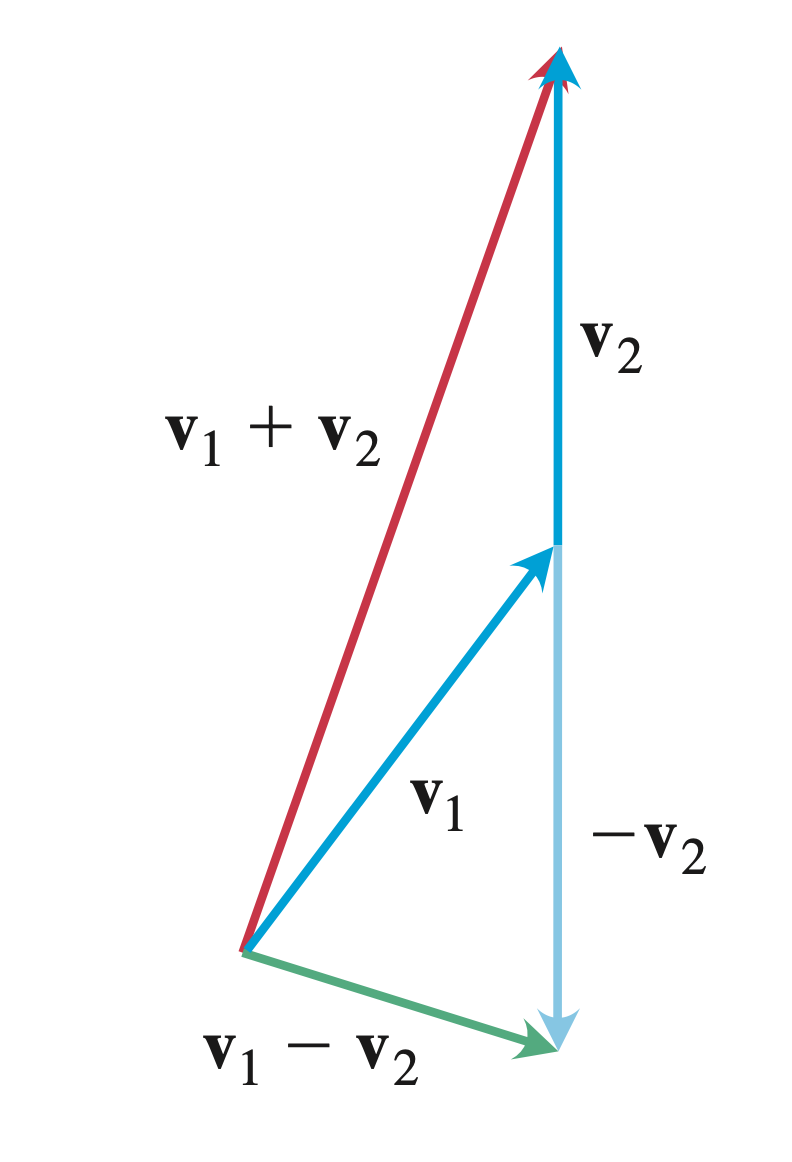
\includegraphics[scale=0.3]{./assets/thomas12.3q19.png}
          \end{center}

          \textbf{Solution.}
          \begin{align*}
              (v_1 + v_2) \cdot (v_1 - v_2) & = v_1 \cdot v_1 - v_1 \cdot v_2 + v_2 \cdot v_1 - v_2 \cdot v_2 \\
                                            & = \lVert v_1 \rVert^2 - \lVert v_2 \rVert^2                     \\
                                            & = 0 \quad (v_1 = v_2)
          \end{align*}
          Therefore, the sum of two vectors is orthogonal to their difference \textbf{if and only if the two vectors are in equal length}. $\hfill\blacksquare$

          \newpage
    \item \textbf{Orthogonality on a circle} Suppose that $A B$ is the diameter of a circle with
          center $O$ and that $C$ is a point on one of the arcs joining $A$ and $B$. Show
          that $\overrightarrow{C A}$ and $\overrightarrow{C B}$ are orthogonal.
          \begin{center}
              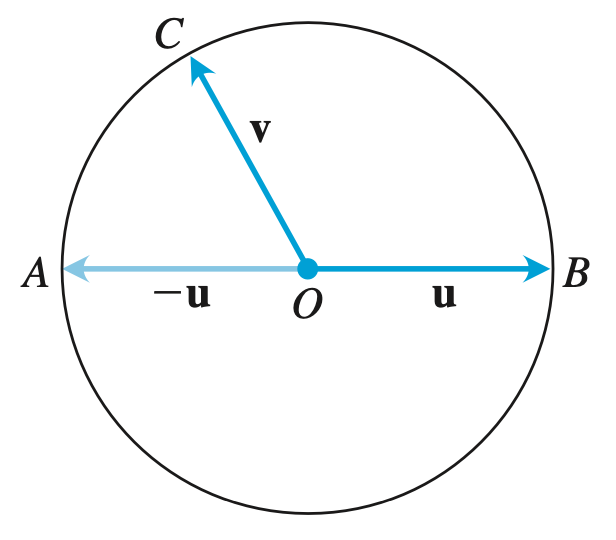
\includegraphics[scale=0.4]{./assets/thomas12.3q20.png}
          \end{center}
          \textbf{Solution. }Since $\lVert u \rVert = \lVert v \rVert = $ radius of the circle, $\overrightarrow{C A} = \overrightarrow{CO} + \overrightarrow{OA} = -u - v$ and $\overrightarrow{C B} = \overrightarrow{CO} + \overrightarrow{OB} = u - v$, we have
          \begin{align*}
              \overrightarrow{C A} \cdot \overrightarrow{C B} & = (-u - v) \cdot (u - v)                               \\
                                                              & = -u \cdot u - u \cdot (-v) - v \cdot u - v \cdot (-v) \\
                                                              & = -\lVert u \rVert^2 + \lVert v \rVert^2               \\
                                                              & = 0
          \end{align*}
          Therefore, $\overrightarrow{C A}$ and $\overrightarrow{C B}$ are orthogonal. $\hfill\blacksquare$

    \item \textbf{Diagonals of a rhombus} Show that the diagonals of a rhombus (parallelogram with
          sides of equal length) are perpendicular.
          \\\textbf{Solution.}
          \begin{center}
              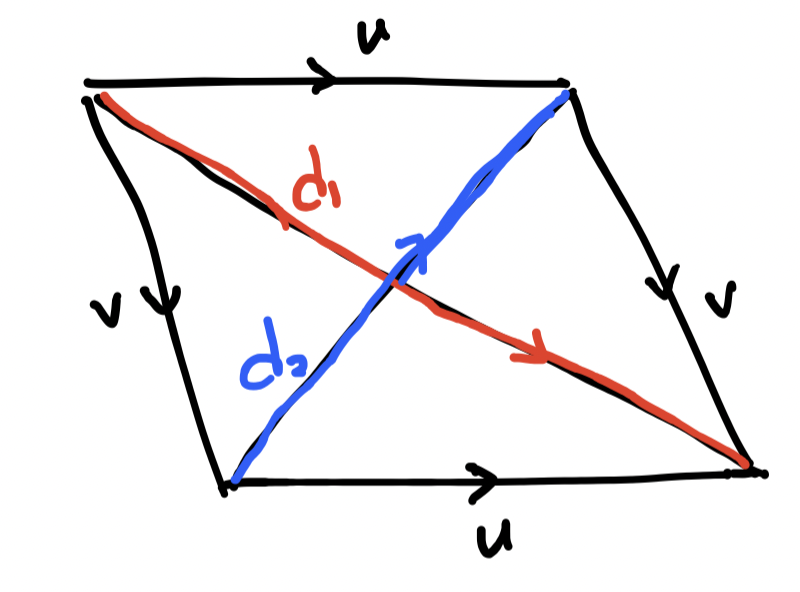
\includegraphics[scale=0.4]{assets/thomas12.3q21.png}
          \end{center}
          Since $d_1 = u + v$ and $d_2 = -v + u$, we have
          \begin{align*}
              d_1 \cdot d_2 & = (u + v) \cdot (-v + u)                        \\
                            & = u \cdot u - u \cdot v + v \cdot u - v \cdot v \\
                            & = \lVert u \rVert^2 - \lVert v \rVert^2         \\
                            & = 0
          \end{align*}
          Therefore, the diagonals of a rhombus are perpendicular. $\hfill\blacksquare$

          \setcounter{enumi}{23}
    \item \textbf{Diagonal of parallelogram} Show that the indicated diagonal of the parallelogram
          determined by vectors $\mathbf{u}$ and $\mathbf{v}$ bisects the angle between
          $\mathbf{u}$ and $\mathbf{v}$ if $|\mathbf{u}|=|\mathbf{v}|$.
          \begin{center}
              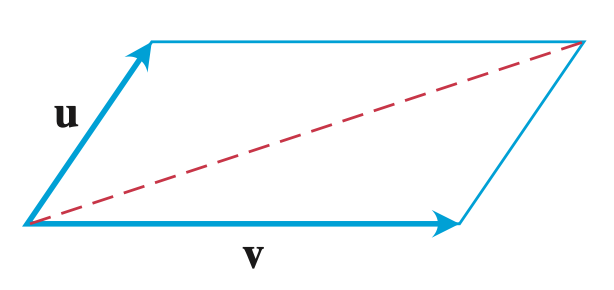
\includegraphics[scale=0.5]{assets/thomas12.3q24.png}
          \end{center}
          \text{Solution. }
          \begin{align*}
              (u + v) \cdot u & = u \cdot u + u \cdot v         \\
                              & = \lVert u \rVert^2 + u \cdot v \\
                              & = \lVert v \rVert^2 + u \cdot v \\
                              & = v \cdot v + u \cdot v         \\
                              & = (u + v) \cdot v
          \end{align*}
          Hence, the angle $\arccos\left(\dfrac{(u + v) \cdot u}{\lVert u + v \rVert \lVert u \rVert}\right)$ between the diagonal and $\vec{u}$ is equal to the angle $\arccos\left(\dfrac{(u + v) \cdot v}{\lVert u + v \rVert \lVert v \rVert}\right)$ between the diagonal and $\vec{v}$ because the inverse cosine function is one-to-one.

          Therefore, the indicated diagonal of the parallelogram determined by vectors
          $\mathbf{u}$ and $\mathbf{v}$ bisects the angle between $\mathbf{u}$ and
          $\mathbf{v}$ if $|\mathbf{u}|=|\mathbf{v}|$. $\hfill\blacksquare$

    \item \textbf{Projectile motion} A gun with muzzle velocity of $400 \mathrm{~m} / \mathrm{s}$ is fired at an angle of $8^{\circ}$ above the horizontal. Find the horizontal and vertical components of the velocity.
          \\\textbf{Solution. }Let $\vec{v + u}$ be the velocity of the bullet, where $\vec{v}$ is the vertical component and $\vec{u}$ is the horizontal component.
          \begin{multicols}{2}
              \begin{center}
                  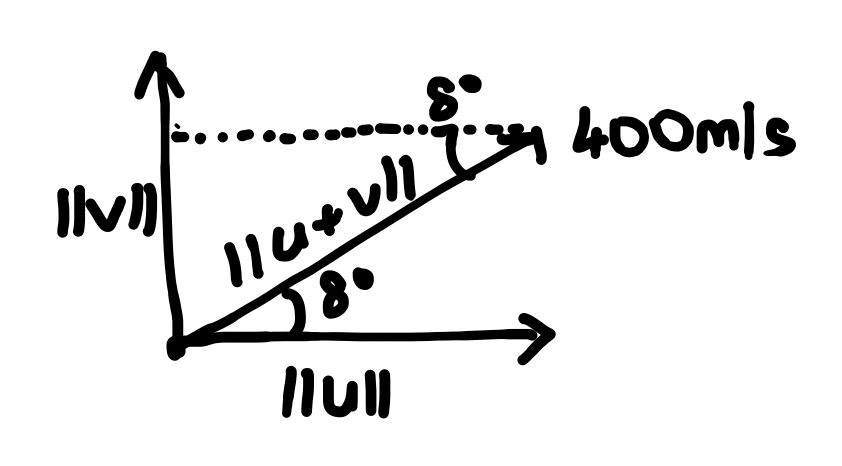
\includegraphics[scale=0.5]{assets/thomas12.3q25.png}
              \end{center}
              \columnbreak
              \begin{align*}
                  \dfrac{\lVert u \lVert}{\lVert u + v \rVert} & = \cos 8^{\circ}                   \\
                  \lVert u \rVert                              & = 400 \cos 8^{\circ}               \\
                                                               & = 396.107 \mathrm{~m} / \mathrm{s}
              \end{align*}

              \begin{align*}
                  \dfrac{\lVert v \lVert}{\lVert u + v \rVert} & = \sin 8^{\circ}                  \\
                  \lVert v \rVert                              & = 400 \sin 8^{\circ}              \\
                                                               & = 55.669 \mathrm{~m} / \mathrm{s}
              \end{align*}
              $\hfill\blacksquare$
          \end{multicols}

    \item \textbf{Inclined plane} Suppose that a box is being towed up an inclined plane as shown in the figure. Find the force $w$ needed to make the component of the force parallel to the inclined plane equal to $2.5 \mathrm{~N}$.
          \begin{center}
              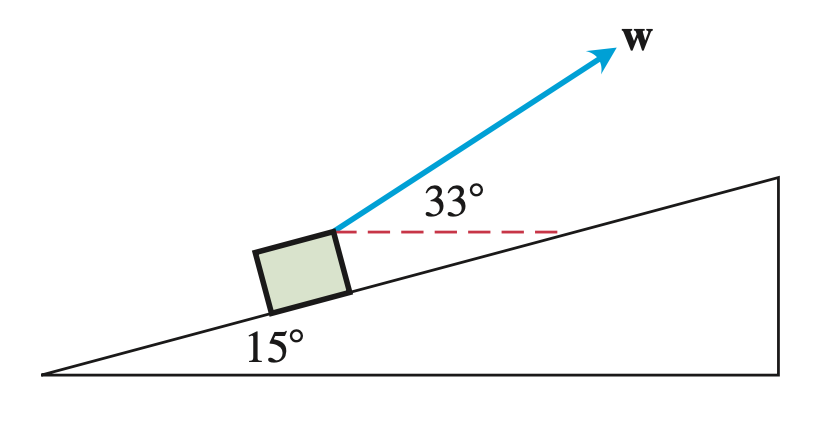
\includegraphics[scale=0.5]{assets/thomas12.3q26.png}
          \end{center}
          \textbf{Solution. }
          \begin{center}
              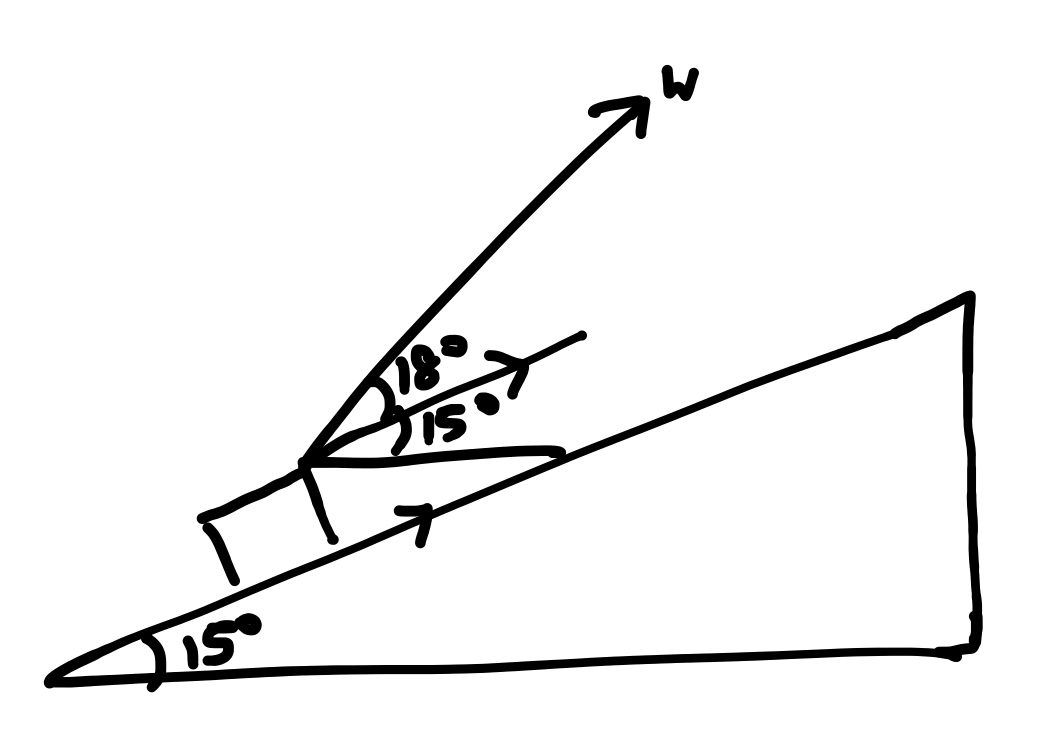
\includegraphics[scale=0.4]{assets/thomas12.3q26sol.png}
          \end{center}
          \begin{align*}
              \lVert w \rVert \cos (33^{\circ} - 15^{\circ}) & = 2.5                          \\
              \lVert w \rVert                                & = \dfrac{2.5}{\cos 18^{\circ}}
          \end{align*}
          \begin{align*}
              w & = \lVert w \rVert \langle \cos 33^{\circ}, \sin 33^{\circ} \rangle             \\
                & =\dfrac{2.5}{\cos 18^{\circ}} \langle \cos 33^{\circ}, \sin 33^{\circ} \rangle \\
                & = \langle 2.205, 1.432 \rangle                                                 \\
          \end{align*}
          $\hfill\blacksquare$

          \newpage
          \setcounter{enumi}{28}
    \item \textbf{Orthogonal unit vectors} If $\mathbf{u}_1$ and $\mathbf{u}_2$ are orthogonal unit vectors and $\mathbf{v}=a \mathbf{u}_1+b \mathbf{u}_2$, find $\mathbf{v} \cdot \mathbf{u}_1$.
          \\\textbf{Solution.}
          \begin{align*}
              \mathbf{v} \cdot \mathbf{u}_1 & = (a \mathbf{u}_1+b \mathbf{u}_2) \cdot \mathbf{u}_1                  \\
                                            & = a \mathbf{u}_1 \cdot \mathbf{u}_1+b \mathbf{u}_2 \cdot \mathbf{u}_1 \\
                                            & = a \lVert \mathbf{u}_1 \rVert^2 + b \mathbf{u}_2 \cdot \mathbf{u}_1  \\
                                            & = a(1) + b(0)                                                         \\
                                            & = a
          \end{align*}
          $\hfill\blacksquare$

    \item A force $\mathbf{F}=2 \mathbf{i}+\mathbf{j}-3 \mathbf{k}$ is applied to a
          spacecraft with velocity vector $\mathbf{v}=3 \mathbf{i}-\mathbf{j}$. Express
          $\mathbf{F}$ as a sum of a vector parallel to $\mathbf{v}$ and a vector
          orthogonal to $\mathbf{v}$. \\\textbf{Solution. } The vector parallel to
          $\mathbf{v}$ is
          \begin{align*}
              \text{proj}_v F & = \left(\dfrac{F \cdot v}{\lVert v \rVert^2}\right)v      \\
                              & = \left(\dfrac{5}{10}\right)(3i - j)                      \\
                              & = \left(\dfrac{3}{2}\right)i - \left(\dfrac{1}{2}\right)j
          \end{align*}
          The vector orthogonal to $\mathbf{v}$ is
          \begin{align*}
              \mathbf{F} - \text{proj}_v F & = \left(2i + j - 3k\right) - \left(\dfrac{3}{2}\right)i + \left(\dfrac{1}{2}\right)j \\
                                           & = \left(\dfrac{1}{2}\right)i + \left(\dfrac{3}{2}\right)j - 3k
          \end{align*}
          $\hfill\blacksquare$

\end{enumerate}

\subsection*{Equations for Lines in the Plane}

\begin{enumerate}
    \setcounter{enumi}{32}
    \item \textbf{Line perpendicular to a vector} Show that $\mathbf{v}=a \mathbf{i}+b \mathbf{j}$ is perpendicular to the line $a x+b y=c$ by establishing that the slope of the vector $\mathbf{v}$ is the negative reciprocal of the slope of the given line.
          \\\textbf{Solution. }Let $P(x_1, y_1)$ and $Q(x_2, y_2)$ be two points on the line $ax + by = c$. Then,
          \begin{align*}
              P(x_1, y_1) & = \left(x_1, \dfrac{c - ax_1}{b}\right) \\
              Q(x_2, y_2) & = \left(x_2, \dfrac{c - ax_2}{b}\right)
          \end{align*}
          \begin{align*}
              \overrightarrow{PQ} & = \left\langle x_2 - x_1, y_2 - y_1 \right\rangle                                 \\
                                  & = \left\langle x_2 - x_1, \dfrac{c - ax_2}{b} - \dfrac{c - ax_1}{b} \right\rangle \\
                                  & = \left\langle x_2 - x_1, \dfrac{a(x_1 - x_2)}{b} \right\rangle
          \end{align*}
          \begin{align*}
              \overrightarrow{PQ} \cdot v & = \left\langle x_2 - x_1, \dfrac{a(x_1 - x_2)}{b} \right\rangle \cdot \left\langle a, b \right\rangle \\
                                          & = a(x_2 - x_1) + \dfrac{a(x_1 - x_2)}{b} \cdot b                                                      \\
                                          & = a(x_2 - x_1) - a(x_2 - x_1)                                                                         \\
                                          & = 0
          \end{align*}
          Therefore, $\mathbf{v}$ is perpendicular to the line $ax + by = c$. $\hfill\blacksquare$
          ~\\\\
          Alternatively, the slope of the vector $\mathbf{v}$ is $\dfrac{b}{a}$, while
          the slope of the line $ax + by = c$ is $-\dfrac{a}{b}$. Therefore, the vector
          $\mathbf{v}$ is perpendicular to the line $ax + by = c$, since slope of the vector $\mathbf{v}$ is the negative reciprocal of the slope of the given line. $\hfill\blacksquare$

    \item \textbf{Line parallel to a vector} Show that the vector $\mathbf{v}=a \mathbf{i}+b \mathbf{j}$ is parallel to the line $b x-a y=c$ by establishing that the slope of the line segment representing $\mathbf{v}$ is the same as the slope of the given line.
          \\\textbf{Solution. }The slope of the vector $v$ is $\dfrac{b}{a}$, while the slope of the given line is also $\dfrac{b}{a}$. Therefore, the vector $\mathbf{v}$ is parallel to the line $bx - ay = c$. $\hfill\blacksquare$
\end{enumerate}

\chapter{Projections}

Given two vectors $\vec{v}$ and $\vec{u}$. Construct a line from the terminal
point of $\vec{u}$ perpendicular to $\vec{v}$. The vector that starts from the
initial point of $\vec{u}$ and ends at the intersection of the line and
$\vec{v}$ is called the \textbf{projection of $\vec{u}$ onto $\vec{v}$}, which
is also known as the \textbf{vector component of $\vec{u}$ along $\vec{v}$}.

Construct another vector from the initial point of $\vec{u}$ that is orthogonal
to $\vec{w_1}$, and the projection of $\vec{u}$ onto that vector is called the
\textbf{vector component of $\vec{u}$ orthogonal to $\vec{v}$}. The visual
representation is shown below.
\begin{center}
    \begin{tikzpicture}[scale=1.8]
        %draw vector u and v
        \draw[->] (0, 0) -- (2, 2);
        \draw[->] (0, 0) -- (3, 0);
        %draw vector w_1, w_2
        \draw[->, thick] (0, 0) -- (2, 0);
        \draw[->, thick] (0, 0) -- (0, 2);
        %draw dashed line
        \draw[-, dashed] (2, 2) -- (2, 0);
        %label vectors
        \node[above left] at (1, 1) {$\vec{u}$};
        \node[below] at (1, 0) {$\vec{w_1}$};
        \node[below] at (2.5, 0) {$\vec{v}$};
        \node[left] at (0, 1) {$\vec{w_2}$};
    \end{tikzpicture}
\end{center}

From the diagram, it is not hard to see that \[\vec{u} = \vec{w_1} + \vec{w_2}\]

Hence, the vector component of $\vec{u}$ orthogonal to $\vec{v}$ is given by \[\vec{w_2} = \vec{u} - \vec{w_1}\]

The projection of $\vec{u}$ onto $\vec{v}$ is given by \[\vec{w_1} = proj_{\vec{v}}\vec{u} = \left(\frac{\vec{u} \cdot \vec{v}}{\lVert \vec{v} \rVert^2}\right)\vec{v}\]

\newpage
\noindent\textbf{Example 1. } Find the projection of $\vec{u} = \langle 6, 7 \rangle$ onto $\vec{v} = \langle 1, 4 \rangle$. Hence, find the vector component of $\vec{u}$ orthogonal to $\vec{v}$.
\begin{align*}
    proj_{\vec{v}}\vec{u} & = \left(\frac{\vec{u} \cdot \vec{v}}{\lVert \vec{v} \rVert^2}\right)\vec{v} \\
                          & = \left(\frac{6(1) + 7(4)}{1^2 + 4^2}\right)\langle 1, 4 \rangle            \\
                          & = \left(\frac{34}{17}\right)\langle 1, 4 \rangle                            \\
                          & = \langle 2, 8 \rangle                                                      \\
    \\
    \vec{w_2}             & = \vec{u} - \vec{w_1}                                                       \\
                          & = \langle 6, 7 \rangle - \langle 2, 8 \rangle                               \\
                          & = \langle 4, -1 \rangle
\end{align*}
\noindent\textbf{Example 2. } Find the projection of $\vec{u} = 2i + 3j$ onto $\vec{v} = 5i + j$. Hence, find the vector component of $\vec{u}$ orthogonal to $\vec{v}$.
\begin{align*}
    proj_{\vec{v}}\vec{u} & = \left(\frac{\vec{u} \cdot \vec{v}}{\lVert \vec{v} \rVert^2}\right)\vec{v}      \\
                          & = \left(\frac{2(5) + 3(1)}{5^2 + 1^2}\right)(5i + j)                             \\
                          & = \left(\frac{13}{26}\right)(5i + j)                                             \\
                          & = \left(\frac{5}{2}\right)i + \left(\frac{1}{2}\right)j                          \\
    \\
    \vec{w_2}             & = \vec{u} - \vec{w_1}                                                            \\
                          & = (2i + 3j) - \left(\left(\frac{5}{2}\right)i + \left(\frac{1}{2}\right)j\right) \\
                          & = \left(-\frac{1}{2}\right)i + \left(\frac{5}{2}\right)j
\end{align*}

\chapter{Direction Cosines and Direction Angles}

\begin{center}
    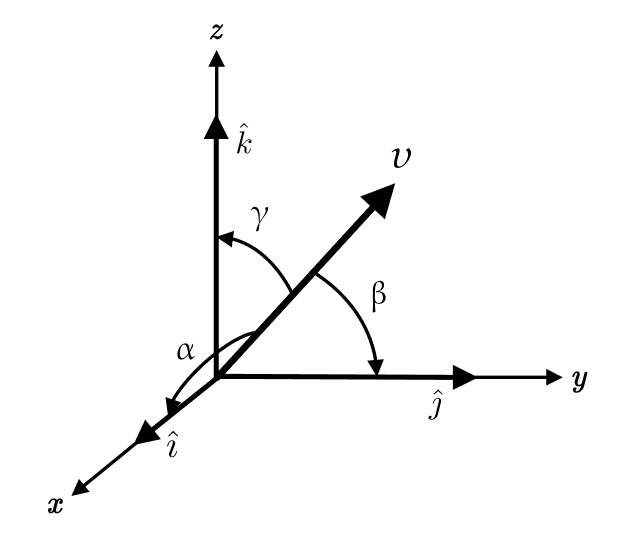
\includegraphics[scale=0.25]{assets/Direction_cosine_vector 1.png}
\end{center}

Direction angles are angles that a vector makes with the unit vectors
$\hat{\imath}$, $\hat{\jmath}$ and $\hat{k}$, denoted by $\alpha$, $\beta$ and
$\gamma$ respectively. In other words, $alpha$, $\beta$ and $\gamma$ are the
angles between the vector and the $x$, $y$ and $z$ axis respectively.

Recall the formula for the dot product of two vectors $\vec{v}$ and $\vec{u}$\[ \vec{v} \cdot \vec{u} = \lVert \vec{v} \rVert \lVert \vec{u} \rVert \cos\theta\] where $\theta$ is the angle between the two vectors.

Let's calculate the dot product of $\vec{v}$ and $\hat{\imath}$.
\begin{align*}
    \vec{v} \cdot \hat{\imath}                                  & = \lVert \vec{v} \rVert \lVert \hat{\imath} \rVert \cos\alpha \\
    \langle v_1, v_2, v_3 \rangle \cdot \langle 1, 0, 0 \rangle & = \lVert \vec{v} \rVert \times 1 \times \cos\alpha            \\
    v_1                                                         & = \lVert \vec{v} \rVert \cos\alpha                            \\
    \cos\alpha                                                  & = \frac{v_1}{\lVert \vec{v} \rVert}
\end{align*}

\newpage
Similarly, we can calculate the dot product of $\vec{v}$ and $\hat{\jmath}$ and
$\hat{k}$ in the same way. Hence, we can conclude that \[\cos\alpha = \frac{v_1}{\lVert \vec{v} \rVert} \qquad \cos\beta = \frac{v_2}{\lVert \vec{v} \rVert} \qquad \cos\gamma = \frac{v_3}{\lVert \vec{v} \rVert}\]
These are called the \textbf{direction cosines} of $\vec{v}$.

We can also express any unit vector $\hat{v}$ in terms of its direction
cosines.
\begin{align*}
    \vec{v}                                & = v_1\hat{\imath} + v_2\hat{\jmath} + v_3\hat{k}                                                                                              \\
    \dfrac{\vec{v}}{\lVert \vec{v} \rVert} & = \dfrac{v_1}{\lVert \vec{v} \rVert}\hat{\imath} + \dfrac{v_2}{\lVert \vec{v} \rVert}\hat{\jmath} + \dfrac{v_3}{\lVert \vec{v} \rVert}\hat{k} \\
    \hat{v}                                & = \cos\alpha\hat{\imath} + \cos\beta\hat{\jmath} + \cos\gamma\hat{k}
\end{align*}
If we take the magnitude of $\hat{v}$, we get \[\lVert \hat{v} \rVert = \sqrt{\cos^2\alpha + \cos^2\beta + \cos^2\gamma} = 1\] Squaring both sides, we get \[\cos^2\alpha + \cos^2\beta + \cos^2\gamma = 1\]
~\\
\noindent\textbf{Example 1. } Find the direction cosines and direction angles of the vector $\vec{u} = \hat{\imath} + 8\hat{\jmath} + 4\hat{k}$.
\begin{align*}
    \lVert \vec{u} \rVert & = \sqrt{1^2 + 8^2 + 4^2} \\
                          & = \sqrt{81}              \\
                          & = 9
\end{align*}
\vspace{-5em}
\begin{multicols}{2}
    \begin{align*}
        \cos\alpha & = \frac{v_1}{\lVert \vec{v} \rVert} = \frac{1}{9} \\
        \cos\beta  & = \frac{v_2}{\lVert \vec{v} \rVert} = \frac{8}{9} \\
        \cos\gamma & = \frac{v_3}{\lVert \vec{v} \rVert} = \frac{4}{9}
    \end{align*}

    \begin{align*}
        \alpha & = \cos^{-1}\left(\frac{1}{9}\right) \approx 1.459 \text{ rad} \\
        \beta  & = \cos^{-1}\left(\frac{8}{9}\right) \approx 0.476 \text{ rad} \\
        \gamma & = \cos^{-1}\left(\frac{4}{9}\right) \approx 1.110 \text{ rad}
    \end{align*}
\end{multicols}

\chapter{Cross Product}

Let $\vec{v} = \langle v_1, v_2, v_3 \rangle$ and $\vec{u} = \langle u_1, u_2,
    u_3 \rangle$ be two vectors in $\mathbb{R}^3$ (three-dimensional space), then
the cross product of $\vec{v}$ and $\vec{u}$ is given by \[\vec{v} \times \vec{u} = (v_2u_3 - v_3u_2)\hat{\imath} + (v_3u_1 - v_1u_3)\hat{\jmath} + (v_1u_2 - v_2u_1)\hat{k}\]
The final result of the cross product is a vector, hence the name
\textbf{vector product}.

It can also be calculated using the determinant of a $3 \times 3$ matrix as
shown below.
\begin{align*}
    \vec{v} \times \vec{u} & = \begin{vmatrix}
                                   \hat{\imath} & \hat{\jmath} & \hat{k} \\
                                   v_1          & v_2          & v_3     \\
                                   u_1          & u_2          & u_3
                               \end{vmatrix}                               \\
                           & = \begin{vmatrix}
                                   v_2 & v_3 \\
                                   u_2 & u_3
                               \end{vmatrix}\hat{\imath} - \begin{vmatrix}
                                                               v_1 & v_3 \\
                                                               u_1 & u_3
                                                           \end{vmatrix}\hat{\jmath} + \begin{vmatrix}
                                                                                           v_1 & v_2 \\
                                                                                           u_1 & u_2
                                                                                       \end{vmatrix}\hat{k}             \\
                           & = (v_2u_3 - v_3u_2)\hat{\imath} - (v_1u_3 - v_3u_1)\hat{\jmath} + (v_1u_2 - v_2u_1)\hat{k}
\end{align*}

Geometrically speaking, the cross product of two vectors $\vec{v}$ and
$\vec{u}$ is a vector that is orthogonal to both $\vec{v}$ and $\vec{u}$, and
its direction is given by the right-hand rule. That is, $\vec{v} \times \vec{u}
    \neq \vec{u} \times \vec{v}$. \vspace{1em}
\begin{center}
    \begin{tikzpicture}
        %draw x, y and z axis
        \draw[->] (0, 0, 0) -- (3, 0, 0);
        \draw[->] (0, 0, 0) -- (0, 3, 0);
        \draw[->] (0, 0, 0) -- (0, 0, 3);
        \node[above] at (1.5, 0, 0) {$\vec{v}$};
        \node[right] at (0, 1.5, 0) {$\vec{u} \times \vec{v}$};
        \node[above left] at (0, 0, 1.5) {$\vec{u}$};
    \end{tikzpicture}
\end{center}

Another property of the cross product is that the magnitude of the cross
product of two vectors $\vec{v}$ and $\vec{u}$ is given by \[\lVert \vec{v} \times \vec{u} \rVert = \lVert \vec{v} \rVert \lVert \vec{u} \rVert \sin\theta\] where $\theta$ is the angle between the two vectors.

The magnitude of the cross product of two vectors $\vec{v}$ and $\vec{u}$ is
the area of the parallelogram formed by $\vec{v}$ and $\vec{u}$. ~\\\\
\noindent\textbf{Proof. } Note that $\cos \theta = \dfrac{\vec{v} \cdot
        \vec{u}}{\lVert \vec{v} \rVert \lVert \vec{u} \rVert}$, hence
\begin{align*}
    \lVert \vec{v} \times \vec{u} \rVert & = \lVert \vec{v} \rVert \lVert \vec{u} \rVert \sin\theta                                                                                          \\
                                         & = \lVert \vec{v} \rVert \lVert \vec{u} \rVert \sqrt{1 - \cos^2\theta}                                                                             \\
                                         & = \lVert \vec{v} \rVert \lVert \vec{u} \rVert \sqrt{1 - \left(\frac{\vec{v} \cdot \vec{u}}{\lVert \vec{v} \rVert \lVert \vec{u} \rVert}\right)^2} \\
                                         & = \sqrt{\lVert \vec{v} \rVert^2 \lVert \vec{u} \rVert^2 - (\vec{v} \cdot \vec{u})^2}                                                              \\
                                         & = \sqrt{(v_1^2 + v_2^2 + v_3^2)(u_1^2 + u_2^2 + u_3^2) - (v_1u_1 + v_2u_2 + v_3u_3)^2}                                                            \\
                                         & = \sqrt{(v_2u_3 - v_3u_2)^2 + (v_3u_1 - v_1u_3)^2 + (v_1u_2 - v_2u_1)^2}                                                                          \\
                                         & = \lVert \vec{v} \times \vec{u} \rVert
\end{align*}
\vspace{0.8em}
\begin{center}
    \begin{tikzpicture}
        \draw[->] (0, 0) -- (2, 2);
        \draw[->] (0, 0) -- (5, 0);
        \draw[-, dashed] (2, 2) -- (7, 2);
        \draw[-, dashed] (5, 0) -- (7, 2);
        \draw[-, dashed] (2, 2) -- (2, 0);
        %label vectors
        \node[above left] at (1, 1) {$\vec{u}$};
        \node[below] at (3.5, 0) {$\vec{v}$};
        %label angles arc
        \draw (0.5, 0) arc (0:45:0.5);
        \node[right] at (0.5, 0.25) {$\theta$};
        %draw curly brace
        \draw [decorate,decoration={brace,mirror,amplitude=5pt},xshift=-4pt,yshift=0pt]
        (2.2, 0) -- (2.2, 2) node [black, right,midway,xshift=0.1cm] {\footnotesize $\lVert \vec{u} \rVert \sin\theta$};
    \end{tikzpicture}
\end{center}
Since the height of the parallelogram is $\lVert \vec{u} \rVert \sin\theta$ and the base of the parallelogram is $\lVert \vec{v} \rVert$, the area of the parallelogram is given By
\begin{align*}
    \text{Area} & = (\text{base})(\text{height})                             \\
                & = \lVert \vec{v} \rVert \lVert \vec{u} \rVert \sin\theta   \\
                & = \lVert \vec{v} \times \vec{u} \rVert \qquad \blacksquare
\end{align*}

\newpage
\noindent\textbf{Example 1. } Find the cross product of the vectors $\vec{v} = \langle 1, 2, 3 \rangle$ and $\vec{u} = \langle -1, 0, 4 \rangle$.
\begin{align*}
    \vec{v} \times \vec{u} & = \begin{vmatrix}
                                   i  & j & k \\
                                   1  & 2 & 3 \\
                                   -1 & 0 & 4
                               \end{vmatrix}                    \\
                           & = \begin{vmatrix}
                                   2 & 3 \\
                                   0 & 4
                               \end{vmatrix}i - \begin{vmatrix}
                                                    1  & 3 \\
                                                    -1 & 4
                                                \end{vmatrix}j + \begin{vmatrix}
                                                                     1  & 2 \\
                                                                     -1 & 0
                                                                 \end{vmatrix}k   \\
                           & = (2(4) - 3(0))i - (1(4) - 3(-1))j + (1(0) - 2(-1))k \\
                           & = 8i - 7j + 2k
\end{align*}
\noindent\textbf{Example 2. } Find the unit vector that is orthogonal to both $\vec{v} = 2i - 3j + k$ and $\vec{u} = i + 2j - k$.
\begin{align*}
    \vec{v} \times \vec{u} & = \begin{vmatrix}
                                   i & j  & k  \\
                                   2 & -3 & 1  \\
                                   1 & 2  & -1
                               \end{vmatrix}                     \\
                           & = \begin{vmatrix}
                                   -3 & 1  \\
                                   2  & -1
                               \end{vmatrix}i - \begin{vmatrix}
                                                    2 & 1  \\
                                                    1 & -1
                                                \end{vmatrix}j + \begin{vmatrix}
                                                                     2 & -3 \\
                                                                     1 & 2
                                                                 \end{vmatrix}k     \\
                           & = (-3(-1) - 1(2))i - (2(-1) - 1(1))j + (2(2) - 1(-3))k \\
                           & = i + 3j + 7k
\end{align*}
\begin{align*}
    \lVert \vec{v} \times \vec{u} \rVert & = \sqrt{1^2 + 3^2 + 7^2} \\
                                         & = \sqrt{59}
\end{align*}
\begin{align*}
    \text{Unit vector} & = \frac{\vec{v} \times \vec{u}}{\lVert \vec{v} \times \vec{u} \rVert} \\
                       & = \frac{1}{\sqrt{59}}i + \frac{3}{\sqrt{59}}j + \frac{7}{\sqrt{59}}k
\end{align*}

\chapter{Distance in Space}

\begin{center}
    \begin{tikzpicture}[scale=0.8]
        %draw x, y and z axis
        \draw[->] (0, 0, 0) -- (5, 0, 0);
        \draw[->] (0, 0, 0) -- (0, 5, 0);
        \draw[->] (0, 0, 0) -- (0, 0, 5);
        %draw point P_1 and P_2
        \draw[fill] (0, 4, 3) circle [radius=0.05];
        \draw[fill] (4, 3, 2) circle [radius=0.05];
        %draw line connecting P_1 and P_2
        \draw[-] (0, 4, 3) -- (4, 3, 2);
        %label point P_1 and P_2
        \node[above] at (0, 4, 3) {$P_1$};
        \node[above] at (4, 3, 2) {$P_2$};
        %label x, y and z axis
        \node[right] at (5, 0, 0) {$y$};
        \node[above] at (0, 5, 0) {$z$};
        \node[below left] at (0, 0, 5) {$x$};
    \end{tikzpicture}
\end{center}
The distance between two points $P_1(x_1, y_1, z_1)$ and $P_2(x_2, y_2, z_2)$
in space is essentially the magnitude of the vector $\overrightarrow{P_1P_2}$,
which is given by \[d = \sqrt{(x_2 - x_1)^2 + (y_2 - y_1)^2 + (z_2 - z_1)^2}\]
~\\
\noindent\textbf{Example 1. } Find the distance between the points $P_1(-3, 2, 5)$ and $P_2(4, 0, 8)$ in space.
\begin{align*}
    d & = \sqrt{(4 - (-3))^2 + (0 - 2)^2 + (8 - 5)^2} \\
      & = \sqrt{7^2 + (-2)^2 + 3^2}                   \\
      & = \sqrt{62}
\end{align*}

\chapter{Lines in Space}

\begin{center}
    \begin{tikzpicture}[scale=0.8]
        %draw x, y and z axis
        \draw[->] (0, 0, 0) -- (5, 0, 0);
        \draw[->] (0, 0, 0) -- (0, 5, 0);
        \draw[->] (0, 0, 0) -- (0, 0, 5);
        %draw point P_1 and P_2
        \draw[fill] (0, 2, 3) circle [radius=0.05];
        \draw[fill] (4, 3, 2) circle [radius=0.05];
        %draw line connecting P_1 and P_2
        \draw[-] (-1, 1.75, 3.25) -- (5, 3.25, 1.75);
        \draw[->, thick] (0, 2, 3) -- (4, 3, 2);
        \draw[->, thick] (0, 0, 0) -- ({8/(3*2^0.5)}, {2/(3*2^0.5)}, {-2/(3*2^0.5)});
        %label point P_1 and P_2
        \node[above left] at (0, 2, 3) {$P(x_1, y_1, z_1)$};
        \node[below right] at (4, 3, 2) {$Q(x_2, y_2, z_2)$};
        %label line
        \node[above left] at (5, 3.25, 1.75) {$L$};
        \node[above] at ({4/(3*2^0.5)}, {1/(3*2^0.5)}, {-1/(3*2^0.5)}) {$\vec{v}$};
        %label x, y and z axis
        \node[right] at (5, 0, 0) {$y$};
        \node[above] at (0, 5, 0) {$z$};
        \node[below left] at (0, 0, 5) {$x$};
    \end{tikzpicture}
\end{center}

To find the equation of a line in space, we need a point $P(x_1, y_1, z_1)$ on
the line and a vector $\vec{v} = \langle a, b, c \rangle$ that is parallel to
the line. The vector $\vec{v}$ is called the \textbf{direction vector} of the
line, while $a$, $b$ and $c$ are called the \textbf{direction numbers}.

Since $\vec{v}$ is parallel to $L$, the vector $\overrightarrow{PQ}$ is also
parallel to $L$, where $Q(x, y, z)$ is any point on $L$. Hence,
$\overrightarrow{PQ}$ is a scalar multiple of $\vec{v}$, that is,
\begin{align*}
    \overrightarrow{PQ}                       & = t\vec{v}                   \\
    \langle x - x_1, y - y_1, z - z_1 \rangle & = t\langle a, b, c \rangle   \\
                                              & = \langle at, bt, ct \rangle
\end{align*}
Comparing both sides, we get \[x - x_1 = at \qquad y - y_1 = bt \qquad z - z_1 = ct\]
Rearranging the equations, we get the \textbf{parametric equations} of the line
$L$. \[x = x_1 + at \qquad y = y_1 + bt \qquad z = z_1 + ct\]

If $a, b, c \neq 0$, we can solve for $t$ for each of the parametric equations
to get the \textbf{symmetric equations} of the line $L$. \[\frac{x - x_1}{a} = \frac{y - y_1}{b} = \frac{z - z_1}{c}\]
~\\
\noindent\textbf{Example 1. } Find the equation of the line that passes through the point $P(-1, 4, 5)$ and is parallel to the vector $\vec{v} = 4i - j$.
\begin{align*}
    x & = -1 + 4t \\
    y & = 4 - t   \\
    z & = 5
\end{align*}
Note that it is impossible to find the symmetric equation of the line since $c = 0$.
~\\\\
\noindent\textbf{Example 2. } $L$ passes through the point $P(2, 7, 1)$ and is parallel to the vector $\vec{v} = \langle -2, -4, 6 \rangle$. Find the parametric and symmetric equations of $L$.
\begin{align*}
    x & = 2 - 2t \\
    y & = 7 - 4t \\
    z & = 1 + 6t
\end{align*}
\begin{align*}
    \frac{x - 2}{-2} & = \frac{y - 7}{-4} = \frac{z - 1}{6}
\end{align*}
\noindent\textbf{Example 3. } Find the equation of the line passing through the point $(1, 0, 1)$ and parallel to the line given by the parametric equations \[x = 3 + 3t \qquad y = 5 - 2t \qquad z = -7 + t\]
The line is parallel to the vector $\vec{v} = \langle 3, -2, 1 \rangle$. Hence,
the equation of the line is given by \[x = 1 + 3t \qquad y = -2t \qquad z = 1 + t\]
Also, the symmetric equations of the line is given by \[\frac{x - 1}{3} = \frac{y}{-2} = \frac{z - 1}{1}\]
\noindent\textbf{Example 4. } Find the equation of the line passing through points $(7, -2, 6)$ and $(-3, 0, 6)$.
\begin{align*}
    \vec{v} & = \langle -3 - 7, 0 - (-2), 6 - 6 \rangle \\
            & = \langle -10, 2, 0 \rangle
\end{align*}
The equation of the line is given by \[x = 7 - 10t \qquad y = -2 + 2t \qquad z = 6\]
There is no symmetric equation of the line since $c = 0$.

\chapter{Planes in Space}

\begin{center}
    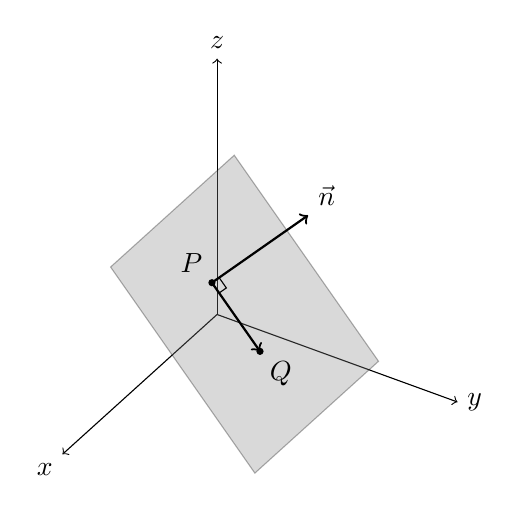
\begin{tikzpicture}[x={({cos(20)},{-sin(20)},0)},z={({-sin(40)},{-cos(40)},0)},scale=0.65]
        %draw x, y and z axis
        \draw[->] (0, 0, 0) -- (5, 0, 0);
        \draw[->] (0, 0, 0) -- (0, 5, 0);
        \draw[->] (0, 0, 0) -- (0, 0, 5);
        %draw a 3d sloped plane
        \draw[-, fill=gray, opacity=0.3] (1, 4, 1) -- (1, 4, 5) -- (4, 1, 5) -- (4, 1, 1) -- cycle;
        % label x, y and z axis
        \node[right] at (5, 0, 0) {$y$};
        \node[above] at (0, 5, 0) {$z$};
        \node[below left] at (0, 0, 5) {$x$};

        \fill (1.5,2.5,2.5) circle (0.2em) node [above left] {$P$};
        \fill (2.5,1.5,2.5) circle (0.2em) node [below right] {$Q$};
        \draw [->, thick] (1.5,2.5,2.5) -- (2.5,1.5,2.5);
        \draw [->, thick] (1.5,2.5,2.5) -- (3.5,4.5,2.5) node [above right] {$\vec{n}$};
        \draw (1.65,2.65,2.5) -- (1.8,2.5,2.5) -- (1.65,2.35,2.5);
    \end{tikzpicture}
\end{center}

To find the equation of a plane in space, we need a point $P(x_1, y_1, z_1)$ on
the plane and a vector $\vec{n} = \langle a, b, c \rangle$ that is orthogonal
to the plane, called the \textbf{normal vector} of the plane.

For any point $Q(x, y, z)$ on the plane, the vector $\overrightarrow{PQ}$ is
orthogonal to $\vec{n}$, that is,
\begin{align*}
    \overrightarrow{PQ} \cdot \vec{n}                                       & = 0 \\
    \langle x - x_1, y - y_1, z - z_1 \rangle \cdot \langle a, b, c \rangle & = 0 \\
    a(x - x_1) + b(y - y_1) + c(z - z_1)                                    & = 0
\end{align*}
This equation is called the \textbf{standard form} of the equation of the plane. Regrouping the terms, we obtain the \textbf{general form} of equation of the plane. \[ax + by + cz + d = 0\] where $d = -ax_1 - by_1 - cz_1$.

\newpage
\noindent\textbf{Example 1. } Find the
equation of the plane that passes through the point $P(4, 5, -7)$ and is
perpendicular to the vector $\vec{n} = \hat{\jmath}$.
\begin{align*}
    \vec{n}                        & = \langle 0, 1, 0 \rangle \\
    0(x - 4) + 1(y - 5) + 0(z + 7) & = 0                       \\
    y - 5                          & = 0                       \\
    y                              & = 5
\end{align*}
\noindent\textbf{Example 2. } Find the
equation of the plane that passes through the point $P(0, 7, 0)$ and is
perpendicular to the vector $\vec{n} = 3\hat{\imath} + 8\hat{k}$.
\begin{align*}
    \vec{n}                        & = \langle 3, 0, 8 \rangle \\
    3(x - 0) + 0(y - 7) + 8(z - 0) & = 0                       \\
    3x + 8z                        & = 0
\end{align*}
\noindent\textbf{Example 3. } Given three points $(0, 0, 0)$, $(2, 0, 7)$, and $(-2, -1, 7)$ in space, find the equation of the plane that passes through these points.
\begin{align*}
    \vec{u} & = \langle 2 - 0, 0 - 0, 7 - 0 \rangle                                                  \\
            & = \langle 2, 0, 7 \rangle                                                              \\
    \vec{v} & = \langle -2 - 0, -1 - 0, 7 - 0 \rangle                                                \\
            & = \langle -2, -1, 7 \rangle                                                            \\
    \vec{n} & = \vec{u} \times \vec{v}                                                               \\
            & = \begin{vmatrix}
                    \hat{\imath} & \hat{\jmath} & \hat{k} \\
                    2            & 0            & 7       \\
                    -2           & -1           & 7
                \end{vmatrix}                           \\
            & = \begin{vmatrix}
                    0  & 7 \\
                    -1 & 7
                \end{vmatrix}\hat{\imath} - \begin{vmatrix}
                                                2  & 7 \\
                                                -2 & 7
                                            \end{vmatrix}\hat{\jmath} + \begin{vmatrix}
                                                                            2  & 0  \\
                                                                            -2 & -1
                                                                        \end{vmatrix}\hat{k}         \\
            & = (0(7) - 7(-1))\hat{\imath} - (2(7) - (-2)(7))\hat{\jmath} + (2(-1) - (-2)(0))\hat{k} \\
            & = 7\hat{\imath} - 28\hat{\jmath} - 2\hat{k}                                            \\
            & = \langle 7, -28, -2 \rangle
\end{align*}
\begin{align*}
    7(x - 0) - 28(y - 0) - 2(z - 0) & = 0 \\
    7x - 28y - 2z                   & = 0
\end{align*}
\newpage
\noindent\textbf{Example 4. } Find the equation of the plane that passes through $(4, 2, 1)$, $(-1, 8, 8)$ and is parallel to $z$-axis.
\begin{align*}
    \vec{v} & = \langle -1 - 4, 8 - 2, 8 - 1 \rangle                                           \\
            & = \langle -5, 6, 7 \rangle                                                       \\
    \vec{n} & = \vec{v} \times \hat{k}                                                         \\
            & = \begin{vmatrix}
                    \hat{\imath} & \hat{\jmath} & \hat{k} \\
                    -5           & 6            & 7       \\
                    0            & 0            & 1
                \end{vmatrix}                     \\
            & = \begin{vmatrix}
                    6 & 7 \\
                    0 & 1
                \end{vmatrix}\hat{\imath} - \begin{vmatrix}
                                                -5 & 7 \\
                                                0  & 1
                                            \end{vmatrix}\hat{\jmath} + \begin{vmatrix}
                                                                            -5 & 6 \\
                                                                            0  & 0
                                                                        \end{vmatrix}\hat{k}   \\
            & = (6(1) - 7(0))\hat{\imath} - (-5(1) - 7(0))\hat{\jmath} + (-5(0) - 6(0))\hat{k} \\
            & = 6\hat{\imath} + 5\hat{\jmath}                                                  \\
            & = \langle 6, 5, 0 \rangle
\end{align*}
\vspace{-3.5em}
\begin{align*}
    6(x - 4) + 5(y - 2) + 0(z - 1) & = 0 \\
    6x + 5y - 34                   & = 0
\end{align*}
\noindent\textbf{Example 5. } Find the equation of the plane such that the point $(2, 0, 1)$ and the line $\dfrac{x}{2} = \dfrac{y-4}{-1} = \dfrac{z}{1}$ is on the plane.
~\\
When $x = 0$, $y = 4$ and $z = 0$, hence the point $(0, 4, 0)$ is on the plane.
\begin{align*}
    \vec{v} & = \langle 2 - 0, 0 - 4, 1 - 0 \rangle                                              \\
            & = \langle 2, -4, 1 \rangle                                                         \\
    \vec{n} & = \langle 2, -1, 1 \rangle \times \langle 2, -4, 1 \rangle                         \\
            & = \begin{vmatrix}
                    \hat{\imath} & \hat{\jmath} & \hat{k} \\
                    2            & -1           & 1       \\
                    2            & -4           & 1
                \end{vmatrix}                       \\
            & = \begin{vmatrix}
                    -1 & 1 \\
                    -4 & 1
                \end{vmatrix}\hat{\imath} - \begin{vmatrix}
                                                2 & 1 \\
                                                2 & 1
                                            \end{vmatrix}\hat{\jmath} + \begin{vmatrix}
                                                                            2 & -1 \\
                                                                            2 & -4
                                                                        \end{vmatrix}\hat{k}     \\
            & = (-1(1) - 1(-4))\hat{\imath} - (2(1) - 2(1))\hat{\jmath} + (2(-4) - 2(-1))\hat{k} \\
            & = -3\hat{\imath} + 0\hat{\jmath} + (-6)\hat{k}                                     \\
            & = \langle -3, 0, -6 \rangle
\end{align*}
\vspace{-3.5em}
\begin{align*}
    -3(x - 2) + 0(y - 0) - 6(z - 1) & = 0 \\
    -3x - 6z + 12                   & = 0
\end{align*}
\newpage
\noindent\textbf{Example 6. } Find the equation of the plane that passes through the points $(3, 4, 1)$ and $(3, 1, -7)$ and is perpendicular to the plane $8x + 9y + 3z  = 13$.
~\\\\
The normal vector of the plane is $\langle 8, 9, 3 \rangle$. Since the target plane is perpendicular to the given plane, the normal vector of the given plane is parallel to the target plane.
\begin{align*}
    \vec{u} & = \langle 8, 9, 3 \rangle                                                          \\
    \vec{v} & = \langle 3 - 3, 1 - 4, -7 - 1 \rangle                                             \\
            & = \langle 0, -3, -8 \rangle                                                        \\
    \vec{n} & = \vec{u} \times \vec{v}                                                           \\
            & = \begin{vmatrix}
                    \hat{\imath} & \hat{\jmath} & \hat{k} \\
                    8            & 9            & 3       \\
                    0            & -3           & -8
                \end{vmatrix}                       \\
            & = \begin{vmatrix}
                    9  & 3  \\
                    -3 & -8
                \end{vmatrix}\hat{\imath} - \begin{vmatrix}
                                                8 & 3  \\
                                                0 & -8
                                            \end{vmatrix}\hat{\jmath} + \begin{vmatrix}
                                                                            8 & 9  \\
                                                                            0 & -3
                                                                        \end{vmatrix}\hat{k}     \\
            & = (9(-8) - 3(-3))\hat{\imath} - (8(-8) - 3(0))\hat{\jmath} + (8(-3) - 9(0))\hat{k} \\
            & = -63\hat{\imath} + 64\hat{\jmath} - 24\hat{k}                                     \\
            & = \langle -63, 64, -24 \rangle
\end{align*}
\vspace{-3.5em}
\begin{align*}
    -63(x - 3) + 64(y - 4) - 24(z - 1) & = 0 \\
    -63x + 64y - 24z - 43              & = 0
\end{align*}

\chapter{Cylindrical Coordinates}

Cylindrical coordinates are an extension of polar coordinates into three
dimensions. A point $P(x, y, z)$ in space is represented by the ordered triple
$(r, \theta, z)$, called the \textbf{cylindrical coordinates} of $P$. Here,
$(r, \theta)$ are the polar representation of the projection of $P$ in the
$xy$-plane, and $z$ is the direct distance from the $(r, \theta)$ to $P$.
\begin{center}
    \tdplotsetmaincoords{60}{110}
    \begin{tikzpicture}[tdplot_main_coords,scale=0.8]
        %draw x, y and z axis
        \draw[->] (0, 0, 0) -- (5, 0, 0);
        \draw[->] (0, 0, 0) -- (0, 5, 0);
        \draw[->] (0, 0, 0) -- (0, 0, 5);
        %draw point P
        \draw[fill] (4, 4, 4) circle [radius=0.05];
        %label point P
        \node[left] at (4, 4, 4) {$P$};
        \node[above=0.5em, right] at (4, 4, 4) {$(x,y,z)$};
        \node[below right] at (4, 4, 4) {$(r,\theta,z)$};
        %draw line connecting P to xy-plane
        \draw[-, dashed] (4, 4, 4) -- (4, 4, 0);
        %draw line connecting P to x-axis
        \draw[-, dashed] (4, 4, 0) -- (4, 0, 0);
        %draw line connecting P to y-axis
        \draw[-, dashed] (4, 4, 0) -- (0, 4, 0);
        %draw line connecting P to origin
        \draw[-, dashed] (4, 4, 0) -- (0, 0, 0) node [above,midway] {$r$};
        %draw arc
        \tdplotdefinepoints(0, 0, 0)(4, 0, 0)(4, 4, 0)
        \tdplotdrawpolytopearc[->,thick]{1}{below}{$\theta$}
        %label x, y and z axis
        \node[below left] at (5, 0, 0) {$x$};
        \node[right] at (0, 5, 0) {$y$};
        \node[above] at (0, 0, 5) {$z$};
        %curly braces for x and y
        \draw [decorate,decoration={brace,mirror,amplitude=5pt},yshift=-5pt]
        (4, 0, 0) -- (4, 4, 0) node [black,midway,below=0.5em] {\footnotesize $y$};
        \draw [decorate,decoration={brace,mirror,amplitude=5pt},xshift=-5pt]
        (0, 0, 0) -- (4, 0, 0) node [black,midway,left=0.6em,above=0.3em] {\footnotesize $x$};
    \end{tikzpicture}
\end{center}

To convert from Cartesian coordinates to cylindrical coordinates, we use the
following equations. \[r^2 = x^2 + y^2 \qquad \tan\theta = \frac{y}{x} \qquad z = z\]

To convert from cylindrical coordinates to Cartesian coordinates, we use the
following equations. \[x = r\cos\theta \qquad y = r\sin\theta \qquad z = z\]

\noindent\textbf{Example 1. } Convert $\left(4, \dfrac{5\pi}{6}, 3\right)$ from cylindrical coordinates to Cartesian coordinates.
\begin{align*}
    x & = r\cos\theta                      \\
      & = 4\cos\left(\frac{5\pi}{6}\right) \\
      & = -2\sqrt{3}                       \\
    y & = r\sin\theta                      \\
      & = 4\sin\left(\frac{5\pi}{6}\right) \\
      & = 2                                \\
    z & = z                                \\
      & = 3
\end{align*}
Hence, $\left(-2\sqrt{3}, 2, 3\right)$ is the Cartesian coordinates of $\left(4, \dfrac{5\pi}{6}, 3\right)$.
~\\\\
\noindent\textbf{Example 2. } Convert $\left(1, \sqrt{3}, 2\right)$ from Cartesian coordinates to cylindrical coordinates.
\begin{align*}
    r      & = \sqrt{x^2 + y^2}                         \\
           & = \sqrt{1^2 + \sqrt{3}^2}                  \\
           & = 2                                        \\
    \theta & = \tan^{-1}\left(\frac{y}{x}\right)        \\
           & = \tan^{-1}\left(\frac{\sqrt{3}}{1}\right) \\
           & = \frac{\pi}{3}                            \\
    z      & = z                                        \\
           & = 2
\end{align*}
Hence, $\left(2, \dfrac{\pi}{3}, 2\right)$ is the cylindrical coordinates of $\left(1, \sqrt{3}, 2\right)$.

\chapter{Spherical Coordinates}

Spherical coordinates are an ordered triple $P = (\rho, \theta, \phi)$, where
$\rho$ is the distance between the origin and $P$ ($\rho \geq 0$ since it is a
distance), $\theta$ is the angle from cylindrical coordinates where $r \geq 0$
and $\phi$ is the angle between the positive $z$-axis and the line segment
$\overrightarrow{OP}$ ($0 \leq \phi \leq \pi$).
\begin{center}
    \tdplotsetmaincoords{60}{110}
    \begin{tikzpicture}[tdplot_main_coords,scale=0.8]
        %draw x, y and z axis
        \draw[->] (0, 0, 0) -- (5, 0, 0);
        \draw[->] (0, 0, 0) -- (0, 5, 0);
        \draw[->] (0, 0, 0) -- (0, 0, 5);
        %draw point P
        \draw[fill] (4, 4, 4) circle [radius=0.05];
        %label point P
        \node[left] at (0, 0, 0) {$O$};
        \node[right] at (4, 4, 4) {$P$};
        \draw[->, thick] (0, 0, 0) -- (4, 4, 4) node [above,midway] {$\rho$};
        \node[above, right=1.2em] at (4, 4, 4) {$(x,y,z)$};
        \node[below=1.4em, right=1.2em] at (4, 4, 4) {$(r,\theta,z)$};
        %draw line connecting P to xy-plane
        \draw[-, dashed] (4, 4, 4) -- (4, 4, 0);
        %draw line connecting P to origin
        \draw[-, dashed] (4, 4, 0) -- (0, 0, 0) node [above,midway] {$r$};
        %draw arc
        \tdplotdefinepoints(0, 0, 0)(4, 0, 0)(4, 4, 0)
        \tdplotdrawpolytopearc[->,thick]{1}{below}{$\theta$}
        \tdplotdefinepoints(0, 0, 0)(0, 0, 4)(4, 4, 4)
        \tdplotdrawpolytopearc[->,thick]{2}{above right}{$\phi$}
        %label x, y and z axis
        \node[below left] at (5, 0, 0) {$x$};
        \node[right] at (0, 5, 0) {$y$};
        \node[above] at (0, 0, 5) {$z$};
    \end{tikzpicture}
\end{center}

To convert from Cartesian coordinates to spherical coordinates, we use the
following equations. \[\rho^2 = x^2 + y^2 + z^2 \qquad \tan\theta = \frac{y}{x} \qquad \cos\phi = \frac{z}{\rho}\]

To convert from spherical coordinates to Cartesian coordinates, we use the
following equations. \[x = \rho\sin\phi\cos\theta \qquad y = \rho\sin\phi\sin\theta \qquad z = \rho\cos\phi\]

\noindent\textbf{Example 1. } Convert $\left(10, \dfrac{\pi}{6}, \dfrac{\pi}{4}\right)$ from spherical coordinates to Cartesian coordinates.
\begin{align*}
    x & = \rho\sin\phi\cos\theta                                         \\
      & = 10\sin\left(\frac{\pi}{4}\right)\cos\left(\frac{\pi}{6}\right) \\
      & = \frac{5\sqrt{6}}{2}                                            \\
    y & = \rho\sin\phi\sin\theta                                         \\
      & = 10\sin\left(\frac{\pi}{4}\right)\sin\left(\frac{\pi}{6}\right) \\
      & = \frac{5\sqrt{2}}{2}                                            \\
    z & = \rho\cos\phi                                                   \\
      & = 10\cos\left(\frac{\pi}{4}\right)                               \\
      & = 5\sqrt{2}
\end{align*}
Hence, $\left(\dfrac{5\sqrt{6}}{2}, \dfrac{5\sqrt{2}}{2}, 5\sqrt{2}\right)$ is the Cartesian coordinates of $\left(10, \dfrac{\pi}{6}, \dfrac{\pi}{4}\right)$.
~\\\\
\noindent\textbf{Example 2. } Convert $\left(-8, -8, \sqrt{19}\right)$ from Cartesian coordinates to spherical coordinates.
\begin{align*}
    \rho   & = \sqrt{x^2 + y^2 + z^2}                                                    \\
           & = \sqrt{(-8)^2 + (-8)^2 + \left(\sqrt{19}\right)^2}                         \\
           & = 7\sqrt{3}                                                                 \\
    \theta & = \tan^{-1}\left(\frac{y}{x}\right)                                         \\
           & = \tan^{-1}\left(\frac{-8}{-8}\right)                                       \\
           & = \frac{5\pi}{4}\ \text{($3^{rd}$ quadrant since $x$ and $y$ are negative)} \\
    \phi   & = \arccos\left(\frac{z}{\rho}\right)                                        \\
           & = \arccos\left(\frac{\sqrt{19}}{7\sqrt{3}}\right)
\end{align*}
Hence, $\left(7\sqrt{3}, \dfrac{5\pi}{4}, \arccos\left(\dfrac{\sqrt{19}}{7\sqrt{3}}\right)\right)$ is the spherical coordinates of $\left(-8, -8, \sqrt{19}\right)$.

\chapter{Vector-valued Functions}

A vector valued-function is a function that maps a real number to a vector. In
the plane, a vector-valued function is given by \[\vec{r}(t) = \langle x(t),
    y(t) \rangle\] and in space, a vector-valued function is given by \[\vec{r}(t) =
    \langle x(t), y(t), z(t) \rangle\]

Note that different functions can give the same curve. For example, \[\vec{r}(t) = \langle \cos t, \sin t \rangle \quad t \in [0, 2\pi]\]
and \[\vec{r}(t) = \langle \cos 2t, \sin 2t \rangle \quad t \in [0, 2\pi]\]
both give the unit circle.

The domain of a vector-valued function $\vec{r}$ is the intersection of the
domains of the component functions $x(t)$, $y(t)$ and $z(t)$. For example,
given a vector-valued function $\vec{r}(t) = \dfrac{1}{t}\hat{\imath} +
    \dfrac{1}{t-1}\hat{\jmath} + \dfrac{1}{\cos t}\hat{k}$ is $(-\infty, 0) \cup
    (0, 1) \cup (1, \infty)$. The domain of each component function is \[D_{x(t)} = (-\infty, 0) \cup (0, \infty) \qquad D_{y(t)} = (-\infty, 1) \cup (1, \infty) \qquad D_{z(t)} = \mathbb{R}\]
Combining the domains of the component functions, we get the domain of the
vector-valued function $\vec{r}(t)$ \[(D_{x(t)} \cap D_{y(t)} \cap D_{z(t)}) = (-\infty, 0) \cup (0, 1) \cup (1, \infty)\]

\newpage
\noindent\textbf{Example 1. } Sketch the vector-valued function $\vec{r}(t) = \langle 2\cos t, -3\sin t \rangle$.
\begin{align*}
    x                                                        & = 2\cos t      \\
    \cos t                                                   & = \frac{x}{2}  \\
    y                                                        & = -3\sin t     \\
    \sin t                                                   & = -\frac{y}{3} \\
    \cos^2t + \sin^2t                                        & = 1            \\
    \left(\frac{x}{2}\right)^2 + \left(-\frac{y}{3}\right)^2 & = 1            \\
    \frac{x^2}{4} + \frac{y^2}{9}                            & = 1
\end{align*}
Hence, the graph of the vector-valued function $\vec{r}(t) = \langle 2\cos t, -3\sin t \rangle$ is an ellipse with major axis of length 6 and minor axis of length 4.

To find the orientation of the function, we can plot points in increasing
values of $t$. \\\\ \noindent When $t = 0$, $\vec{r}(0) = \langle 2\cos 0,
    -3\sin 0 \rangle = \langle 2, 0 \rangle$. \\\\ \noindent When $t =
    \dfrac{\pi}{2}$, $\vec{r}\left(\dfrac{\pi}{2}\right) = \langle 2\cos
    \dfrac{\pi}{2}, -3\sin \dfrac{\pi}{2} \rangle = \langle 0, -3 \rangle$. \\\\
\noindent Hence, the orientation of the function is clockwise. \vspace{2em}
\begin{center}
    \begin{tikzpicture}[scale=0.8]
        %draw x and y axis
        \draw[->] (-3, 0) -- (3, 0) node [right] {$x$};
        \draw[->] (0, -4) -- (0, 4) node [above] {$y$};
        %draw ellipse
        \draw[thick] (0, 0) ellipse (2 and 3) [arrow inside one={opt={scale=1.5}}{0.12,0.4,0.6,0.92}];
        %draw points
        \fill (2, 0) circle (0.05) node [below right] {$2$};
        \fill (-2, 0) circle (0.05) node [below left] {$-2$};
        \fill (0, 3) circle (0.05) node [above right] {$3$};
        \fill (0, -3) circle (0.05) node [below right] {$-3$};
    \end{tikzpicture}
\end{center}
\newpage
\noindent\textbf{Example 2. } Sketch the vector-valued function $\vec{r}(t) = \dfrac{t}{8}\hat{\imath} + (t - 1)\hat{\jmath}$.
\begin{align*}
    x  & = \frac{t}{8} \\
    t  & = 8x          \\
    \\
    y  & = t - 1       \\
    t  & = y + 1       \\
    \\
    8x & = y + 1       \\
    y  & = 8x - 1
\end{align*}
Hence, the graph of the vector-valued function $\vec{r}(t) = \dfrac{t}{8}\hat{\imath} + (t - 1)\hat{\jmath}$ is a line with $y$-intercept of $-1$ and slope of $8$.
\\\\
When $t = 0$, $\vec{r}(0) = \dfrac{0}{8}\hat{\imath} + (0 - 1)\hat{\jmath} = <0, -1>$. \\\\ When $t = 8$, $\vec{r}(8) = \dfrac{8}{8}\hat{\imath} + (8 - 1)\hat{\jmath} = <1, 7>$. \\\\ Hence, the orientation of the function is going up.
\vspace{1em}
\begin{center}
    \begin{tikzpicture}[scale=0.8]
        %draw x and y axis
        \draw[->] (-3, 0) -- (3, 0) node [right] {$x$};
        \draw[->] (0, -2) -- (0, 8) node [above] {$y$};
        %draw line
        \draw[thick] (-1/8, -2) -- (7/8, 8) [arrow inside one={opt={scale=1.5}}{0.1, 0.2, 0.3, 0.4, 0.5, 0.6, 0.7, 0.8, 0.92}];
        %draw points
        \fill (0, -1) circle (0.05) node [left] {$-1$};
        \fill (0, 7) circle (0.05) node [left] {$7$};
    \end{tikzpicture}
\end{center}

\newpage

\noindent\textbf{Example 3. } Represent $y = x + 9$ as vector-valued function.
\begin{align*}
    x          & = t                                   \\
    y          & = t + 9                               \\
    \vec{r}(t) & = x(t)\hat{\imath} + y(t)\hat{\jmath} \\
               & = t\hat{\imath} + (t+9)\hat{\jmath}
\end{align*}
\noindent\textbf{Example 4. } Represent $x^2 + y^2 = 64$ as vector-valued function.
\begin{align*}
    x          & = 8\cos{t}                                    \\
    y          & = 8\sin{t}                                    \\
    \vec{r}(t) & =x(t)\hat{\imath} + y(t)\hat{\jmath}          \\
               & = 8\cos{t}\hat{\imath} + 8\sin{t}\hat{\jmath}
\end{align*}
\noindent\textbf{Example 5. } Represent $(x-2)^2 + (y + 1)^2 = 4$ as vector-valued function.
\begin{align*}
    2\cos{t}   & = x - 2                                                   \\
    x          & = 2\cos{t} + 2                                            \\
    2\sin{t}   & = y + 1                                                   \\
    y          & = 2\sin{t} - 1                                            \\
    \vec{r}(t) & = x(t)\hat{\imath} + y(t)\hat{\jmath}                     \\
               & = (2\cos{t} + 2)\hat{\imath} + (2\sin{t} - 1)\hat{\jmath}
\end{align*}
Hence, we can conclude that the vector-valued function of a circle with radius $r$ and centre $(h, k)$ is \[\vec{r}(t) = (h + r\cos{t})\hat{\imath} + (k + r\sin{t})\hat{\jmath}\]
\noindent\textbf{Example 6. } Represent $\dfrac{x^2}{9}+ \dfrac{y^2}{4} = 1$ as vector-valued function.
\begin{align*}
    x          & = 3\cos{t}                                    \\
    y          & = 2\sin{t}                                    \\
    \vec{r}(t) & = x(t)\hat{\imath} + y(t)\hat{\jmath}         \\
               & = 3\cos{t}\hat{\imath} + 2\sin{t}\hat{\jmath}
\end{align*}
\noindent\textbf{Example 7. } Represent $\dfrac{(x-1)^2}{4}+ \dfrac{(y+2)^2}{25} = 1$ as vector-valued function.
\begin{align*}
    x - 1      & = 2\cos{t}                                                \\
    x          & = 2\cos{t} + 1                                            \\
    y + 2      & = 5\sin{t}                                                \\
    y          & = 5\sin{t} - 2                                            \\
    \vec{r}(t) & = x(t)\hat{\imath} + y(t)\hat{\jmath}                     \\
               & = (2\cos{t} + 1)\hat{\imath} + (5\sin{t} - 2)\hat{\jmath}
\end{align*}
Hence, we can conclude that the vector-valued function of an ellipse with major axis of length $2a$ and minor axis of length $2b$ is \[\vec{r}(t) = (h + a\cos{t})\hat{\imath} + (k + b\sin{t})\hat{\jmath}\]
\noindent\textbf{Example 8. } Represent $\dfrac{x^2}{25} - \dfrac{y^2}{16} = 1$ as vector-valued function.
\begin{align*}
    x          & = 5\cosh{t}                                     \\
    y          & = 4\sinh{t}                                     \\
    \vec{r}(t) & = x(t)\hat{\imath} + y(t)\hat{\jmath}           \\
               & = 5\cosh{t}\hat{\imath} + 4\sinh{t}\hat{\jmath}
\end{align*}
\noindent\textbf{Example 9. } Represent $\dfrac{(x-1)^2}{4} - \dfrac{(y+7)^2}{9} = 1$ as vector-valued function.
\begin{align*}
    x - 1      & = 2\cosh{t}                                                 \\
    x          & = 2\cosh{t} + 1                                             \\
    y + 7      & = 3\sinh{t}                                                 \\
    y          & = 3\sinh{t} - 7                                             \\
    \vec{r}(t) & = x(t)\hat{\imath} + y(t)\hat{\jmath}                       \\
               & = (2\cosh{t} + 1)\hat{\imath} + (3\sinh{t} - 7)\hat{\jmath}
\end{align*}
Hence, we can conclude that the vector-valued function of a hyperbola with centre $(h, k)$ is \[\vec{r}(t) = (h + a\cosh{t})\hat{\imath} + (k + b\sinh{t})\hat{\jmath}\]

\chapter{Limits of Vector-valued Functions}

The limit of a vector-valued function $\vec{r}(t) = \langle x(t), y(t), z(t)
    \rangle$ as $t$ approaches $a$ is
\begin{align*}
    \lim_{t \to a} \vec{r}(t) & = \langle\lim_{t \to a} x(t), \lim_{t \to a} y(t), \lim_{t \to a} z(t) \rangle                   \\
                              & = \lim_{t \to a} x(t)\hat{\imath} + \lim_{t \to a} y(t)\hat{\jmath} + \lim_{t \to a} z(t)\hat{k}
\end{align*}
\noindent\textbf{Example 1. } Find $\lim\limits_{t \to \pi}(t\hat{\imath} + \cos t\hat{\jmath} + \sin t\hat{k})$.
\begin{align*}
    \lim_{t \to \pi} (t\hat{\imath} + \cos t\hat{\jmath} + \sin t\hat{k}) & = \lim_{t \to \pi} t\hat{\imath} + \lim_{t \to \pi} \cos t\hat{\jmath} + \lim_{t \to \pi} \sin t\hat{k} \\
                                                                          & = \pi\hat{\imath} + \cos \pi\hat{\jmath} + \sin \pi\hat{k}                                              \\
                                                                          & = \pi\hat{\imath} - \hat{\jmath}
\end{align*}
\noindent\textbf{Example 2. } Find $\lim\limits_{t \to 0}(e^{6t}\hat{\imath} + \dfrac{\sin{2t}}{2t}\hat{\jmath} + e^{-5t}\hat{k})$.
\begin{align*}
    \lim_{t \to 0} (e^{6t}\hat{\imath} + \dfrac{\sin{2t}}{2t}\hat{\jmath} + e^{-5t}\hat{k}) & = \lim_{t \to 0} e^{6t}\hat{\imath} + \lim_{t \to 0} \dfrac{\sin{2t}}{2t}\hat{\jmath} + \lim_{t \to 0} e^{-5t}\hat{k} \\
                                                                                            & = 1\hat{\imath} + 1\hat{\jmath} + 1\hat{k}                                                                            \\
                                                                                            & = \hat{\imath} + \hat{\jmath} + \hat{k}
\end{align*}
\noindent\textbf{Example 3. } Find $\lim\limits_{t \to \infty}(e^{-t}\hat{\imath} + \dfrac{1}{t^2 + 7}\hat{\jmath} + e^{\arctan{t}}\hat{k})$.
\begin{align*}
    \lim_{t \to \infty} (e^{-t}\hat{\imath} + \dfrac{1}{t^2 + 7}\hat{\jmath} + e^{\arctan{t}}\hat{k}) & = \lim_{t \to \infty} e^{-t}\hat{\imath} + \lim_{t \to \infty} \dfrac{1}{t^2 + 7}\hat{\jmath} + \lim_{t \to \infty} e^{\arctan{t}}\hat{k} \\
                                                                                                      & = 0\hat{\imath} + 0\hat{\jmath} + e^{\frac{\pi}{2}}\hat{k}                                                                                \\
                                                                                                      & = e^{\frac{\pi}{2}}\hat{k}
\end{align*}

\chapter{Derivatives and Integration of Vector-valued Functions}

The derivative of a vector-valued function $\vec{r}(t) = x(t)\hat{\imath} +
    y(t)\hat{\jmath} + z(t)\hat{k}$ is \[\vec{r}'(t) = x'(t)\hat{\imath} +
    y'(t)\hat{\jmath} + z'(t)\hat{k}\]

The indefinite integral of a vector-valued function $\vec{r}(t) =
    x(t)\hat{\imath} + y(t)\hat{\jmath} + z(t)\hat{k}$ is \[\int \vec{r}(t)\ dt = \int x(t)\hat{\imath} + \int y(t)\hat{\jmath} + \int z(t)\hat{k} + C\]

The definite integral of a vector-valued function $\vec{r}(t) =
    x(t)\hat{\imath} + y(t)\hat{\jmath} + z(t)\hat{k}$ from $a$ to $b$ is \[\int_a^b \vec{r}(t)\ dt = \int_a^b x(t)\hat{\imath} + \int_a^b y(t)\hat{\jmath} + \int_a^b z(t)\hat{k}\]

Since this topic is relatively straightforward, there will be no examples. :)

\chapter{Velocity, Speed and Acceleration}

If $x(t)$, $y(t)$ and $z(t)$ are differentiable functions, then the velocity of
a vector-valued function $\vec{r}(t) = x(t)\hat{\imath} + y(t)\hat{\jmath} +
    z(t)\hat{k}$ is \[\vec{v}(t) = (\vec{r})'(t) = x'(t)\hat{\imath} + y'(t)\hat{\jmath} + z'(t)\hat{k}\]

The speed of a vector-valued function $\vec{r}(t) = x(t)\hat{\imath} +
    y(t)\hat{\jmath} + z(t)\hat{k}$ is \[|\vec{v}(t)| = \sqrt{x'(t)^2 + y'(t)^2 + z'(t)^2}\]

The acceleration of a vector-valued function $\vec{r}(t) = x(t)\hat{\imath} +
    y(t)\hat{\jmath} + z(t)\hat{k}$ is \[\vec{a}(t) = (\vec{v})'(t) = x''(t)\hat{\imath} + y''(t)\hat{\jmath} + z''(t)\hat{k}\]

The path of a projectile launched from an initial height $h$ with initial speed
$v_0$ at an angle of elevation $\theta$ is given by \[\vec{r}(t) = v_0\cos\theta t\hat{\imath} + \left[h + (v_0\sin\theta) t - \frac{1}{2}gt^2\right]\hat{\jmath}\]

Since this topic is relatively straightforward also, there will be no examples.
:)

\newpage

\section*{Application Exercises}
\textit{Source: Larson Calculus 11th Ed. Exercise 12.3}

\subsection*{Projectile Motion}
In Exercises 27-32, use the model for projectile motion, assuming there is no
air resistance and $g=9.8$ meters per second per second.
\begin{enumerate}
    \setcounter{enumi}{26}
    \item  A baseball is hit from a height of 1 meter above the ground with an initial
          speed of 40 feet per second and at an angle of $22^{\circ}$ above the
          horizontal. Find the maximum height reached by the baseball. Determine whether
          it will clear a 3-meters-high fence located 105 meters from home plate.

          \textbf{Solution} Given that $h = 1$, $v_0 = 40$, $\theta = 22^{\circ}$ and $g = 9.8$,
          \begin{align*}
              \vec{r}(t) & = v_0\cos\theta t\hat{\imath} + \left[h + (v_0\sin\theta) t - \frac{1}{2}gt^2\right]\hat{\jmath}               \\
                         & = 40\cos{22^{\circ}} t\hat{\imath} + \left[1 + (40\sin{22^{\circ}}) t - \frac{1}{2}(9.8)t^2\right]\hat{\jmath}
          \end{align*}
          The velocity vector is
          \begin{align*}
              \vec{v}(t) & = (\vec{r})'(t) = 40\cos{22^{\circ}}\hat{\imath} + (40\sin{22^{\circ}} - 9.8t)\hat{\jmath}
          \end{align*}
          The maximum height is reached when the vertical component of the velocity is $0$.
          \begin{align*}
              40\sin{22^{\circ}} - 9.8t & = 0 \implies t = \frac{40\sin{22^{\circ}}}{9.8} \approx 1.53\ \text{seconds}
          \end{align*}
          The maximum height is
          \begin{align*}
              y & = 1 + (40\sin{22^{\circ}})\left(\frac{40\sin{22^{\circ}}}{9.8}\right) - \frac{1}{2}(9.8)\left(\frac{40\sin{22^{\circ}}}{9.8}\right)^2 \\
                & \approx 12.46\ \text{meters}
          \end{align*}
          The ball is 105 meters from home plate when $x(t) = 105$.
          \begin{align*}
              40\cos{22^{\circ}} t & = 105 \implies t = \frac{105}{40\cos{22^{\circ}}}  \approx 2.83\ \text{seconds}
          \end{align*}
          At this time, the height of the ball is
          \begin{align*}
              y & = 1 + (40\sin{22^{\circ}})\left(\frac{105}{40\cos{22^{\circ}}}\right) - \frac{1}{2}(9.8)\left(\frac{105}{40\cos{22^{\circ}}}\right)^2 \\
                & \approx 4.15\ \text{meters}
          \end{align*}
          Hence, the ball will clear the fence. \hfill$\blacksquare$

    \item Determine the maximum height and range of a projectile fired at a height of 2
          meters above the ground with an initial speed of 300 meters per second and at
          angle of $45^{\circ}$ above the horizontal.

          \textbf{Solution} Given that $h = 2$, $v_0 = 300$, $\theta = 45^{\circ}$ and $g = 9.8$,
          \begin{align*}
              \vec{r}(t) & = v_0\cos\theta t\hat{\imath} + \left[h + (v_0\sin\theta) t - \frac{1}{2}gt^2\right]\hat{\jmath}                 \\
                         & = 300\cos{45^{\circ}} t\hat{\imath} + \left[2 + (300\sin{45^{\circ}}) t - \frac{1}{2}(9.8)t^2\right]\hat{\jmath} \\
                         & = 150\sqrt{2} t\hat{\imath} + \left[2 + 150\sqrt{2} t - 4.9t^2\right]\hat{\jmath}
          \end{align*}
          The velocity vector is
          \begin{align*}
              \vec{v}(t) & = (\vec{r})'(t)                                              \\
                         & = 150\sqrt{2}\hat{\imath} + (150\sqrt{2} - 9.8t)\hat{\jmath}
          \end{align*}
          The maximum height is reached when the vertical component of the velocity is $0$.
          \begin{align*}
              150\sqrt{2} - 9.8t & = 0                           \\
              t                  & = \frac{150\sqrt{2}}{9.8}     \\
                                 & \approx 21.65\ \text{seconds}
          \end{align*}
          The maximum height is
          \begin{align*}
              y & = 2 + (150\sqrt{2})\left(\frac{150\sqrt{2}}{9.8}\right) - 4.9\left(\frac{150\sqrt{2}}{9.8}\right)^2 \\
                & \approx 2,297.92\ \text{meters}
          \end{align*}
          The projectile hits the ground when $y(t) = 0$.
          \begin{align*}
              2 + (150\sqrt{2}) t - 4.9t^2 & = 0                                                           \\
              t                            & = \frac{-150\sqrt{2} - \sqrt{150^2(2) - 4(-4.9)(2)}}{2(-4.9)} \\
                                           & \approx 43.302\ \text{seconds}
          \end{align*}
          Hence, the range is
          \begin{align*}
              x & = 150\sqrt{2} \left(\frac{-150\sqrt{2} - \sqrt{150^2(2) - 4(-4.9)(2)}}{2(-4.9)}\right) \\
                & \approx 9185.67\ \text{meters}
          \end{align*} \hfill$\blacksquare$

          \newpage
    \item A baseball, hit 1 meter above the ground, leaves the bat at an angle of
          $45^{\circ}$ and is caught by an outfielder 1 feet above the ground and 100
          feet from home plate. What is the initial speed of the ball, and how high does
          it rise?

          \textbf{Solution} Given that $h = 1$, $\theta = 45^{\circ}$ and $g = 9.8$,
          \begin{align*}
              \vec{r}(t) & = v_0\cos\theta t\hat{\imath} + \left[h + (v_0\sin\theta) t - \frac{1}{2}gt^2\right]\hat{\jmath}                 \\
                         & = v_0\cos{45^{\circ}} t\hat{\imath} + \left[1 + (v_0\sin{45^{\circ}}) t - \frac{1}{2}(9.8)t^2\right]\hat{\jmath} \\
                         & = \frac{v_0}{\sqrt{2}} t\hat{\imath} + \left[1 + \frac{v_0}{\sqrt{2}} t - 4.9t^2\right]\hat{\jmath}
          \end{align*}
          When the ball is caught, $x(t) = 100$ and $y(t) = 1$.
          \begin{align*}
              \frac{v_0}{\sqrt{2}} t & = 100 \implies t = \frac{100\sqrt{2}}{v_0}\ \cdots\ (1)
          \end{align*}
          \vspace{-2.4em}
          \begin{align*}
              1 + \frac{v_0}{\sqrt{2}} t - 4.9t^2 & = 1                                     \\
              4.9t^2 - \frac{v_0}{\sqrt{2}} t     & = 0                                     \\
              t(4.9t - \frac{v_0}{\sqrt{2}})      & = 0                                     \\
              t                                   & = \frac{v_0}{4.9\sqrt{2}} \ \cdots\ (2)
          \end{align*}
          Equating $(1)$ and $(2)$,
          \begin{align*}
              \frac{100\sqrt{2}}{v_0} & = \frac{v_0}{4.9\sqrt{2}}                                  \\
              v_0^2                   & = 980                                                      \\
              v_0                     & = 14\sqrt{5}\ \text{meters per second}\ \text{($v_0 > 0$)}
          \end{align*}
          Hence,
          \begin{align*}
              \vec{r}(t) & = \frac{14\sqrt{5}}{\sqrt{2}} t\hat{\imath} + \left[1 + \frac{14\sqrt{5}}{\sqrt{2}} t - 4.9t^2\right]\hat{\jmath} \\
                         & = 7\sqrt{10} t\hat{\imath} + \left[1 + 7\sqrt{10} t - 4.9t^2\right]\hat{\jmath}
          \end{align*}
          The maximum height is reached when the vertical component of the velocity is $0$.
          \begin{align*}
              7\sqrt{10} - 9.8t & = 0                          \\
              t                 & = \frac{7\sqrt{10}}{9.8}     \\
                                & \approx 2.26\ \text{seconds}
          \end{align*}
          The maximum height is
          \begin{align*}
              y & = 1 + (7\sqrt{10})\left(\frac{7\sqrt{10}}{9.8}\right) - 4.9\left(\frac{7\sqrt{10}}{9.8}\right)^2 \\
                & = 26\ \text{meters}
          \end{align*} \hfill$\blacksquare$

    \item A baseball player at second base throws a ball 28 meters to the player at first
          base. The ball is released at a point 1.5 meters above the ground with an
          initial speed of 80 kilometres per hour and at an angle of $15^{\circ}$ above
          the horizontal. At what height does the player at first base catch the ball?

          \textbf{Solution} Given that $h = 1.5$, $v_0 = 80$km/h$=80\times\dfrac{1000}{3600}=22\dfrac{2}{9}$m/s, $\theta = 15^{\circ}$ and $g = 9.8$,
          \begin{align*}
              \vec{r}(t) & = v_0\cos\theta t\hat{\imath} + \left[h + (v_0\sin\theta) t - \frac{1}{2}gt^2\right]\hat{\jmath}                                         \\
                         & = 22\dfrac{2}{9}\cos{15^{\circ}} t\hat{\imath} + \left[1.5 + (22\dfrac{2}{9}\sin{15^{\circ}}) t - \frac{1}{2}(9.8)t^2\right]\hat{\jmath} \\
                         & = 22\dfrac{2}{9}\cos{15^{\circ}} t\hat{\imath} + \left[1.5 + 22\dfrac{2}{9}\sin{15^{\circ}} t - 4.9t^2\right]\hat{\jmath}
          \end{align*}
          When the ball is caught, $x(t) = 28$
          \begin{align*}
              22\dfrac{2}{9}\cos{15^{\circ}} t & = 28 \implies t = \frac{28}{22\dfrac{2}{9}\cos{15^{\circ}}} \approx 1.305\ \text{seconds}
          \end{align*}
          The height of the ball is
          \begin{align*}
              y & = 1.5 + 22\dfrac{2}{9}\sin{15^{\circ}} \left(\frac{28}{22\dfrac{2}{9}\cos{15^{\circ}}}\right) - 4.9\left(\frac{28}{22\dfrac{2}{9}\cos{15^{\circ}}}\right)^2 \\
                & \approx 0.66\ \text{meters}
          \end{align*} \hfill$\blacksquare$

          \newpage
    \item Eliminate the parameter $t$ from the position vector for the motion of a
          projectile to show that the rectangular equation is $$ y=-\frac{g \sec ^2
                  \theta}{2 v_0^2} x^2+(\tan \theta) x+h $$

          \textbf{Solution}
          \begin{align*}
              \vec{r}(t) & = v_0\cos\theta t\hat{\imath} + \left[h + (v_0\sin\theta) t - \frac{1}{2}gt^2\right]\hat{\jmath}
          \end{align*}
          Let $x = v_0\cos\theta t$ and $y = h + (v_0\sin\theta) t - \dfrac{1}{2}gt^2$.
          \begin{align*}
              x & = v_0\cos\theta t                                                                                               \\
              t & = \frac{x}{v_0\cos\theta}                                                                                       \\
              y & = h + (v_0\sin\theta) t - \frac{1}{2}gt^2                                                                       \\
                & = h + (v_0\sin\theta) \left(\frac{x}{v_0\cos\theta}\right) - \frac{1}{2}g\left(\frac{x}{v_0\cos\theta}\right)^2 \\
                & = h + \frac{v_0\sin\theta}{v_0\cos\theta} x - \frac{1}{2}\frac{g}{v_0^2\cos^2\theta} x^2                        \\
                & = h + (\tan\theta) x - \frac{1}{2}\frac{g}{v_0^2\cos^2\theta} x^2                                               \\
                & = -\frac{g \sec ^2 \theta}{2 v_0^2} x^2+(\tan \theta) x+h
          \end{align*} \hfill$\blacksquare$

    \item The path of a ball is given by the rectangular equation $$ y=x-0.0245 x^2 \text
              {. } $$ Use the result of Exercise 31 to find the position vector. Then find
          the speed and direction of the ball at the point at which it has travelled 15
          meters horizontally.

          \textbf{Solution} Comparing the equation with the equation in Exercise 31,
          \begin{align*}
              \tan \theta                       & = 1                                                \\
              \theta                            & = 45^{\circ}                                       \\
              -\frac{g \sec ^2 \theta}{2 v_0^2} & = -0.0245                                          \\
              \frac{9.8}{v_0^2}                 & = 0.0245                                           \\
              v_0^2                             & = 400                                              \\
              v_0                               & = 20\ \text{meters per second}\ \text{($v_0 > 0$)}
          \end{align*}
          Hence, the position vector is
          \begin{align*}
              \vec{r}(t) & = v_0\cos\theta t\hat{\imath} + \left[h + (v_0\sin\theta) t - \frac{1}{2}gt^2\right]\hat{\jmath}               \\
                         & = 20\cos{45^{\circ}} t\hat{\imath} + \left[0 + (20\sin{45^{\circ}}) t - \frac{1}{2}(9.8)t^2\right]\hat{\jmath} \\
                         & = 10\sqrt{2} t\hat{\imath} + \left[10\sqrt{2} t - 4.9t^2\right]\hat{\jmath}
          \end{align*}
          The time taken to travel 15 meters horizontally is
          \begin{align*}
              10\sqrt{2} t & = 15 \implies t = \frac{3\sqrt{2}}{2} \approx 2.12\ \text{seconds}
          \end{align*}
          The speed vector is
          \begin{align*}
              \vec{v}(t) & = (\vec{r})'(t) = 10\sqrt{2}\hat{\imath} + (10\sqrt{2} - 9.8t)\hat{\jmath}
          \end{align*}
          The direction of the ball is
          \begin{align*}
              \vec{v}\left(\frac{3\sqrt{2}}{2}\right) & = 10\sqrt{2}\hat{\imath} + (10\sqrt{2} - 9.8\left(\frac{3\sqrt{2}}{2}\right))\hat{\jmath} \\
                                                      & = 10\sqrt{2}\hat{\imath} - 14.7\sqrt{2}\hat{\jmath}
          \end{align*}
          Hence, the speed of the ball is
          \begin{align*}
              \lVert\vec{v}\left(\frac{3\sqrt{2}}{2}\right)\rVert & = \sqrt{(10\sqrt{2})^2 + (-14.7\sqrt{2})^2} \\
                                                                  & = 25.14\ \text{meters per second}
          \end{align*} \hfill$\blacksquare$
\end{enumerate}

\newpage

\chapter {Tangent Vectors and Normal Vectors}

Let $C$ be a smooth curve represented by $\vec{r}(t) = x(t)\hat{\imath} +
    y(t)\hat{\jmath} + z(t)\hat{k}$ on an open interval $I$, the unit tangent
vector at $t = a$ is a vector that is tangent to the curve at $t = a$ and has a
magnitude of $1$. The unit tangent vector is given by \[\vec{T}(t) = \frac{(\vec{r})'(t)}{\lVert(\vec{r})'(t)\rVert} = \frac{x'(t)\hat{\imath} + y'(t)\hat{\jmath} + z'(t)\hat{k}}{\sqrt{x'(t)^2 + y'(t)^2 + z'(t)^2}}, \quad (\vec{r})'(t) \neq \vec{0}\]

\end{document}